\documentclass[11pt,a4paper]{article}

% Network Security Incidents laboratory - student report (pdfLaTeX / Overleaf / Tectonic).
\usepackage[T1]{fontenc}
\usepackage[utf8]{inputenc}
\usepackage{lmodern}
\usepackage[margin=2.1cm]{geometry}
\usepackage{microtype}
\usepackage{parskip}
\usepackage{amsmath,amssymb}
\usepackage{booktabs}
\usepackage{tabularx}
\usepackage{array}
\usepackage{float}
\usepackage{graphicx}
\usepackage{tikz}
\usetikzlibrary{arrows.meta,positioning}
\usepackage{needspace}
\usepackage{enumitem}
\usepackage{xcolor}
\usepackage{fancyvrb}
\usepackage{cite}
\renewcommand{\citepunct}{], [}
\renewcommand{\citedash}{]--[}
\usepackage{xurl}
\usepackage{hyperref}
\hypersetup{colorlinks=true, linkcolor=blue!50!black, urlcolor=blue!60!black, citecolor=blue!50!black,
  pdftitle={Network Security Incidents: An Investigation Laboratory}, pdfauthor={Diellart Mulolli}}
\setlist{itemsep=0.2em, topsep=0.3em}
\setlength{\emergencystretch}{2em}
\newcolumntype{L}{>{\raggedright\arraybackslash}X}
\newcolumntype{P}[1]{>{\raggedright\arraybackslash}p{#1}}
\newcommand{\code}[1]{\texttt{#1}}

\title{\textbf{Network Security Incidents: An Investigation Laboratory}\\[0.3em]
\large Orange España, HTTP/2 Rapid Reset, Operation RoundPress, the Cisco ASA campaign, Storm-0558 and the xz backdoor}
\author{Diellart Mulolli (230756200035)\\[0.2em] \small Code and LaTeX source: \url{https://github.com/Diellart-Mulolli/network_lab}}
\date{\today}

% ---------------------------------------------------------------- typeset reference diagrams
\newcommand{\fourdiagram}{%
\resizebox{0.98\linewidth}{!}{%
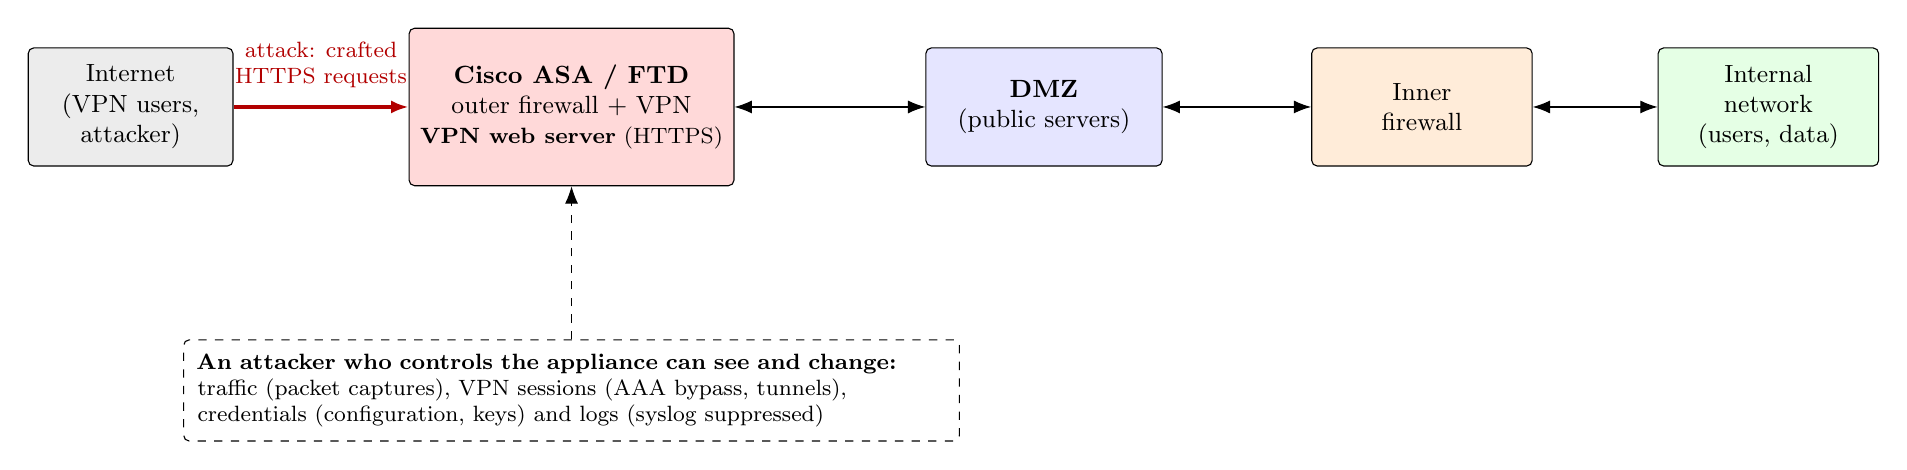
\begin{tikzpicture}[font=\small, >={Latex[length=2.2mm]},
  box/.style={draw, rounded corners=2pt, align=center, minimum height=1.5cm, inner sep=4pt},
  note/.style={draw, dashed, rounded corners=2pt, align=left, inner sep=5pt, font=\footnotesize}]
\node[box, fill=gray!15, minimum width=2.6cm] (inet) at (0,0) {Internet\\(VPN users,\\attacker)};
\node[box, fill=red!15, minimum width=4cm, minimum height=2cm] (fw) at (5.6,0) {\textbf{Cisco ASA / FTD}\\outer firewall + VPN\\{\footnotesize \textbf{VPN web server} (HTTPS)}};
\node[box, fill=blue!10, minimum width=3cm] (dmz) at (11.6,0) {\textbf{DMZ}\\(public servers)};
\node[box, fill=orange!15, minimum width=2.8cm] (ifw) at (16.4,0) {Inner\\firewall};
\node[box, fill=green!10, minimum width=2.8cm] (int) at (20.8,0) {Internal\\network\\(users, data)};
\draw[->, very thick, red!70!black] (inet) -- node[above=3pt, align=center, font=\footnotesize]{attack: crafted\\HTTPS requests} (fw);
\draw[<->] (fw) -- (dmz);
\draw[<->] (dmz) -- (ifw);
\draw[<->] (ifw) -- (int);
\node[note, text width=9.5cm] (ctl) at (5.6,-3.6) {\textbf{An attacker who controls the appliance can see and change:}\\
traffic (packet captures), VPN sessions (AAA bypass, tunnels),\\
credentials (configuration, keys) and logs (syslog suppressed)};
\draw[->, dashed] (ctl.north) -- (fw.south);
\end{tikzpicture}}}

\newcommand{\xzdiagram}{%
\resizebox{0.98\linewidth}{!}{%
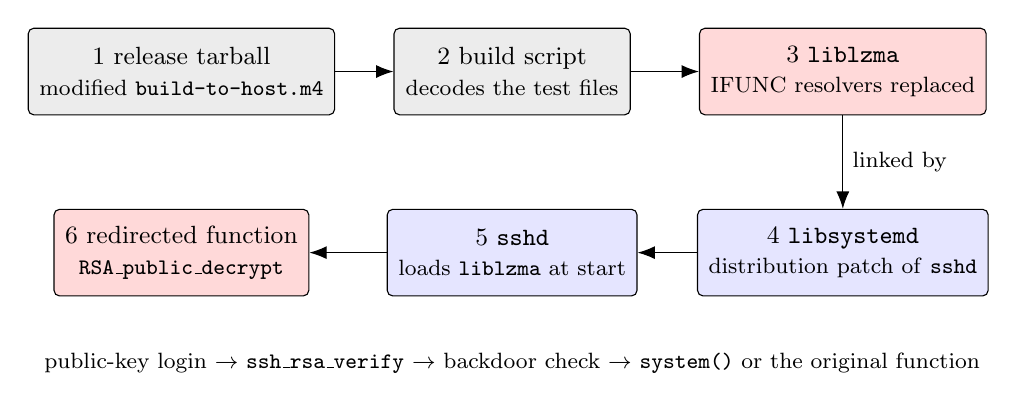
\begin{tikzpicture}[font=\small, >={Latex[length=2.2mm]},
  box/.style={draw, rounded corners=2pt, align=center, minimum height=1.1cm, minimum width=3cm, inner sep=4pt}]
\node[box, fill=gray!15] (tar) at (0,0) {1\ release tarball\\{\footnotesize modified \texttt{build-to-host.m4}}};
\node[box, fill=gray!15] (cfg) at (4.2,0) {2\ build script\\{\footnotesize decodes the test files}};
\node[box, fill=red!15] (lib) at (8.4,0) {3\ \texttt{liblzma}\\{\footnotesize IFUNC resolvers replaced}};
\node[box, fill=blue!10] (sd) at (8.4,-2.3) {4\ \texttt{libsystemd}\\{\footnotesize distribution patch of \texttt{sshd}}};
\node[box, fill=blue!10] (ssh) at (4.2,-2.3) {5\ \texttt{sshd}\\{\footnotesize loads \texttt{liblzma} at start}};
\node[box, fill=red!15] (rsa) at (0,-2.3) {6\ redirected function\\{\footnotesize \texttt{RSA\_public\_decrypt}}};
\draw[->] (tar) -- (cfg); \draw[->] (cfg) -- (lib);
\draw[->] (lib) -- node[right, font=\footnotesize]{linked by} (sd);
\draw[->] (sd) -- (ssh); \draw[->] (ssh) -- (rsa);
\node[align=center, font=\footnotesize] at (4.2,-3.7) {public-key login $\rightarrow$ \texttt{ssh\_rsa\_verify} $\rightarrow$ backdoor check $\rightarrow$ \texttt{system()} or the original function};
\end{tikzpicture}}}

\begin{document}
\maketitle

\section*{Introduction}
Network security failures rarely come from broken mathematics. They come from a protocol feature that costs the
attacker almost nothing (a cancelled request), from a sanitiser that misses one attribute (an e-mail that runs
script), from a signing key that lives too long, or from a build script that nobody read. This laboratory investigates the six real incidents of the laboratory sheet, from 2023 to 2025, one or two for each of its four segments. For every incident
the report identifies the people and products involved from primary sources (vendor and agency posts, a government
review, the original mailing-list post, CVE records), builds a dated timeline, explains the mechanism with the
protocol-level concepts of the course (Stamp, chs.~8--9 \cite{stamp}), and does the required calculations.
All six cases are answered (Table~\ref{tab:cases}).
\begin{table}[H]
\centering\small
\begin{tabularx}{\textwidth}{@{}P{3.6cm}P{2.1cm}L@{}}
\toprule
Segment & Question & Incident \\
\midrule
2.1 Routing and denial of service & Q1, Q2 & Orange España and the hijacked RPKI account (Jan.\ 2024); HTTP/2 Rapid Reset (2023) \\
2.2 Web applications & Q3 & Operation RoundPress, webmail XSS (2023--2024) \\
2.3 Firewalls and intrusion detection & Q4, Q5 & the Cisco ASA firewall campaign (2024--2025); Storm-0558 and the forged key (2023) \\
2.4 Authentication protocols & Q6 & the backdoor in xz and SSH (2024) \\
\bottomrule
\end{tabularx}
\caption{The questions of the sheet and the incidents.}\label{tab:cases}
\end{table}

\paragraph{Method.} The facts were collected from primary sources on the web. Every source is cited by number and listed
with its URL in the reference list (the links are clickable in the PDF); the file \code{SOURCES.md} of the repository lists,
for each source, the facts that were taken from it. The calculations, the route-validation example and the date arithmetic are in four small
Python scripts (Appendices~A.1--A.4) whose output is printed verbatim. The screenshots of Question~1(d) were taken from RIPEstat on 17~November 2026.
The code, the LaTeX source and a running guide are in \url{https://github.com/Diellart-Mulolli/network_lab}. Two questions ask for a drawing made \emph{by hand}
(Questions~4(b) and~6(b)); the scripts cannot produce a drawing on paper, so each figure is a typeset reference diagram that shows what the drawing must
contain, and it is replaced by the photograph of a hand drawing as soon as the file exists (see the captions).

%=====================================================================
\section*{2.1 Routing and Denial of Service}

\subsection*{Question 1 --- When the security mechanism becomes the weapon (3 January 2024)}

\paragraph{(a) The operator, the statements, the analysis, the timeline.} The operator is \textbf{Orange España}
(Orange Spain), autonomous system \textbf{AS12479} (holder name in the RIPE Database: ``UNI2-AS Orange Espagne SA'')
\cite{ripestat}. On 3~January 2024 an attacker logged in to the operator's account at its Regional Internet Registry,
the RIPE NCC, and published Route Origin Authorizations (ROAs) that turned the operator's own routes RPKI-invalid.
\begin{itemize}
\item \emph{The operator's statement.} Orange said on social media that the incident ``affected some of our customers'', that
service was ``practically restored'' by the evening, that no client data had been compromised and that only the browsing of some
services was affected \cite{record}.
\item \emph{The registry's statement.} The RIPE NCC said it was investigating the compromise of the account, which ``resulted in
some services of the account holder being temporarily impacted'', that it had restored access to the legitimate holder, and that it
was ``expediting the 2FA implementation'' for all RIPE NCC Access accounts \cite{record}. Its update of 10~January 2024 decided that
two-factor authentication would become mandatory \cite{ripeupdate}.
\item \emph{The technical analysis} is by Doug Madory of Kentik, a network-measurement company, published on the APNIC blog on
26~January 2024 \cite{apnic}. Cloudflare's measurement of a 50\% fall in Orange España's traffic is reported by The Record
\cite{record}.
\end{itemize}
\begin{table}[H]
\centering\small
\begin{tabular}{@{}llP{11.2cm}@{}}
\toprule
\# & Time (UTC) & Event \\
\midrule
1 & 3 Jan.\ 09:28 & someone, presumably the attacker, starts publishing and revoking ROAs for Orange's address ranges \cite{apnic} \\
2 & 3 Jan.\ 09:42 & three ROAs with origin AS12479 are published, among them 149.74.0.0/16 with maxLength 16 \cite{apnic} \\
3 & 3 Jan.\ about 14:20 & \textbf{impact starts}: ROAs with the wrong origin AS49581 for 85.48.0.0/12 and 90.160.0.0/12 (maxLength 12) and two /21s;
inbound traffic to AS12479 falls until about 18:00 \cite{apnic} \\
4 & 3 Jan.\ just before 18:00 & \textbf{Orange regains control} of the account and publishes ROAs for AS12479 whose maxLength equals the prefix length \cite{apnic} \\
5 & 4 Jan. & over a thousand routes of AS12479 are still RPKI-invalid \cite{apnic} \\
6 & 8 Jan.\ 16:00 & Orange raises the maxLength of the two /12s and the /16 to 24 \cite{apnic} \\
7 & 10 Jan. & the RIPE NCC announces that two-factor authentication will become mandatory \cite{ripeupdate} \\
\bottomrule
\end{tabular}
\caption{Timeline of the Orange España incident (Appendix~A.4: the attack ROAs of 14:20 lasted 3.7~hours; 8.5~hours from the first ROA
activity to the recovery; about 5 days until the maxLength fix).}\label{tab:q1time}
\end{table}

\paragraph{(b) How a security mechanism became the weapon.} The steps, with the validation rules of RFC~6811 \cite{rfc6811}:
\begin{enumerate}[label=\arabic*.]
\item A ROA states that one autonomous system may originate a prefix up to a maximum length. A router that performs
\emph{route origin validation} (ROV) puts every received BGP route into one of three states: \textbf{Valid} (a ROA covers the prefix,
the route is not longer than its maxLength, and the origin AS matches), \textbf{Invalid} (a ROA covers the prefix but none matches) or
\textbf{NotFound} (no ROA covers it) \cite{rfc6811}.
\item The attacker, logged in as Orange, published ROAs naming a different origin, AS49581, for Orange's prefixes (for example the
two /12 blocks 85.48.0.0/12 and 90.160.0.0/12) \cite{apnic}.
\item Orange's real announcements, with origin AS12479, are now \emph{covered} by a ROA, but the only ROA that covers them names AS49581. So
every one of them is \textbf{Invalid}. Orange never changed a route; the data against which routes are judged changed (the phases of
Appendix~A.1).
\item \emph{Only networks that perform ROV drop Invalid routes}; a network without ROV accepts every route. Backbone carriers that do
validation stopped carrying much of Orange's address space, and Kentik had shown earlier that a route evaluated as Invalid has its
propagation cut in half or more \cite{apnic}. The announcements stayed correct, but a large part of the Internet no longer accepted them.
\end{enumerate}
\emph{How much became unreachable.} Kentik's measurements \cite{apnic}: the number of globally routed routes originated by AS12479 fell from
about 9\,200 to about 7\,400 (a loss of about 1\,800, or 19.6\%); the number of unique IPv4 addresses originated fell from about 7~million to
about 5~million (28.6\%, 2~million addresses); inbound traffic fell strongly from about 14:20 to 18:00, and Cloudflare saw about half of
Orange España's traffic disappear for roughly three hours \cite{record}.

\emph{Why some routes stayed invalid for days: the maxLength field.} When Orange regained the account it published ROAs for AS12479
with a maxLength equal to the prefix length: 12 for the two /12s and 16 for 62.36.0.0/16 \cite{apnic}. A route longer than the maxLength is
Invalid even if its origin is correct. Many of Orange's real announcements are /24s inside these blocks (today RIPEstat lists 8\,253 announced prefixes for AS12479, many of them /24s \cite{ripestat}), so over a thousand routes stayed Invalid. They remained reachable only because the covering /12
and /16 were Valid. On 8~January at 16:00 UTC Orange raised the maxLength to 24, and the routes became Valid \cite{apnic}.
Appendix~A.1 reproduces this with the RFC~6811 rules: an announced 85.48.12.0/24 is Invalid under the attacker's ROAs, still
Invalid under a ROA with maxLength 12, and Valid with maxLength 24. The author of the analysis recommends leaving maxLength empty, which
matches the best current practice of RFC~9319 \cite{apnic,rfc9319}.

\paragraph{(c) The authentication failure.} \emph{How the credentials were obtained.} The password reportedly was ``ripeadmin''. APNIC writes
that it had been found in a public leak of stolen credentials \cite{apnic}. Hudson Rock, quoted by The Register, said with ``high certainty'' that
the account of an Orange employee had been in infostealer logs since August 2023 and called the password ridiculously weak \cite{register}.
Orange has not publicly confirmed the method. \emph{The missing protection} was \textbf{two-factor authentication}: it was not enabled on the
account, and the RIPE NCC did not require it, although the American registry ARIN had required it since February 2023 \cite{register}.

\emph{What the registry changed afterwards} \cite{ripeupdate,ripereport}: the RIPE NCC forced password resets on 800 accounts found vulnerable
through leaked credentials (January 2024); it made two-factor authentication mandatory for all RIPE NCC Access accounts; it required longer
passwords and added lock-out against brute force; it automated password resets for credentials found in public breaches; administrators of a
member can see which of their users have not enabled two-factor authentication; and the e-mail address of an account can no longer be changed. Its
investigation counted 870 accounts with publicly exposed passwords, 104 of them linked to LIR accounts, and 270 accounts whose e-mail
address had been changed \cite{ripereport}.

\emph{Should an RPKI account be protected more strongly than an ordinary web account?} Yes, for four reasons. (1) The blast radius is not
the account holder's own data but the reachability of a whole network: one login cost a mobile and broadband operator about a fifth of its globally routed routes and, for hours, about half of its traffic. (2) The change acts on the global routing system: it is enforced by other organisations' routers that the operator cannot
reach or fix, and a bogus ROA with a chosen origin even makes an attacker's own announcement Valid (Appendix~A.1). (3) The account is used
rarely, so strong friction costs little. (4) The recovery is slow: the maxLength mistake showed that repairing ROAs took five days. The proportionate
controls are phishing-resistant second factors (hardware keys) for every user with ROA rights, no password-only access, alerts to several
people when a ROA is created or changed, a short delay or a second approver for changes that make existing routes Invalid, and an alarm
when the validation state of one's own prefixes changes. A counter-argument is that stronger factors increase the risk of lock-out during an
emergency; a break-glass procedure with a physical token held by two people answers it.

\paragraph{(d) Today: the RPKI status of two prefixes.} Using RIPEstat on 17~November 2026 (data as of 16:00 UTC, queries at about 21:50 UTC):
\begin{table}[H]
\centering\small
\begin{tabularx}{\textwidth}{@{}P{3.4cm}P{2.8cm}P{4.1cm}L@{}}
\toprule
Prefix & Origin AS (holder) & ROA found (RIPEstat, validator Routinator) & Status \\
\midrule
85.48.0.0/12 (originated by the operator of Question~1) & AS12479 (Orange Espagne SA) & origin AS12479, \textbf{maxLength 24} &
valid \\
91.187.96.0/19 (a Kosovo provider) & AS21246 (IPKO Telecommunications LLC, Prishtina, Republic of Kosovo) & origin AS21246, \textbf{maxLength 19} &
valid \\
\bottomrule
\end{tabularx}
\caption{ROAs found on 17 November 2026 \cite{ripestat}.}\label{tab:q1today}
\end{table}
The first prefix is one of the blocks attacked in 2024 and its ROA has the maxLength 24 that Orange set on 8~January 2024. The second belongs to IPKO,
the provider with its registered address in Prishtina (the organisation object in the RIPE Database gives the address ``Prishtina, Republic of Kosovo''; its country
attribute is ``AL'', as for the other IPKO objects) \cite{ripestat}. Its ROA allows exactly the /19, so a more specific announcement of the /19 would be
Invalid. Screenshots (Figures~\ref{fig:orangeshot} and~\ref{fig:ipkoshot}) show RIPEstat's overview of each prefix with its date and the RPKI
validation response of the RIPEstat data API with its query time. (In the overview, the RPKI badge of the Orange prefix is yellow and that of the IPKO prefix is
green; the API reports both as valid, and I did not find a description of the badge colours, so the table relies on the API.)
\begin{figure}[H]
\centering
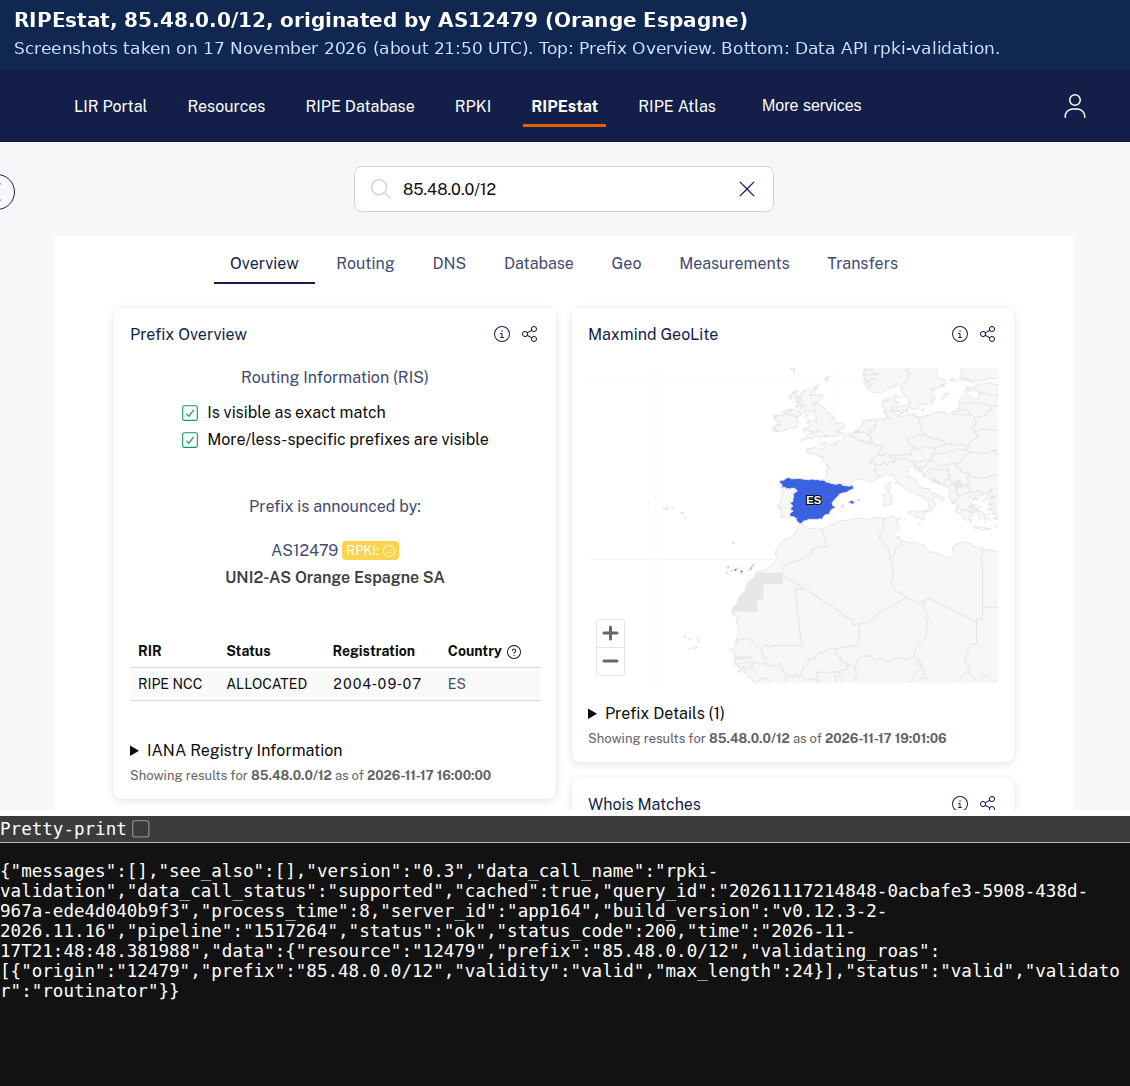
\includegraphics[width=0.88\linewidth]{figures/q1_orange_ripestat.png}
\caption{RIPEstat on 17 November 2026: 85.48.0.0/12, origin AS12479 (Orange España).}\label{fig:orangeshot}
\end{figure}
\begin{figure}[H]
\centering
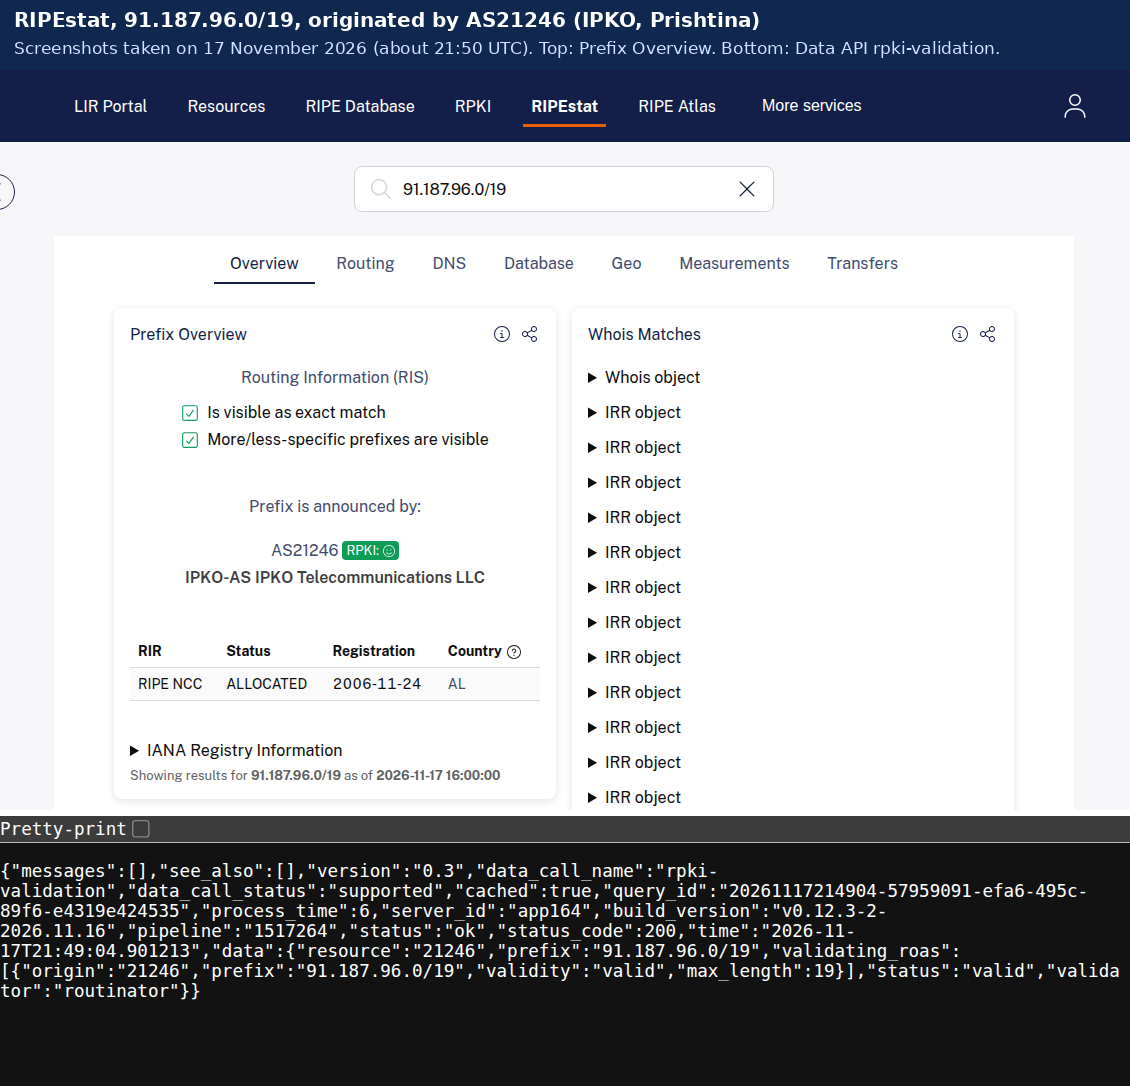
\includegraphics[width=0.88\linewidth]{figures/q1_ipko_ripestat.png}
\caption{RIPEstat on 17 November 2026: 91.187.96.0/19, origin AS21246 (IPKO, Prishtina).}\label{fig:ipkoshot}
\end{figure}
\emph{What an attacker who took over the IPKO registry account could do.} With the account the attacker can create, change and delete the provider's ROAs. The attacker could
(1) publish a ROA naming another AS as origin or delete the correct ROA and add a narrower one: IPKO's announcements become Invalid and every network that does ROV drops
them, an outage like Orange's; (2) publish a ROA that names \emph{the attacker's own} AS: a hijack announced from that AS is then Valid, while IPKO's real route is Invalid, so
validating networks would prefer the attacker's route; (3) raise the maxLength (for example from 19 to 24): then forged-origin announcements of
more specific /24s that keep IPKO's AS as origin become Valid, which is the weakness that RFC~9319 warns about \cite{rfc9319}.

\emph{What the attacker could not do, and what changes if no ROA exists.} The account is not a router: the attacker cannot announce a route without a BGP session and a transit
provider that carries it, cannot read or alter traffic alone, and cannot affect networks that do not do ROV. If \emph{no ROA exists} for a prefix, every announcement
is NotFound, ROV networks accept it, and the attacker cannot make the operator's routes disappear by deleting anything; there is nothing to revoke
and no protection to remove. Absence of a ROA, however, does not protect against account takeover: the attacker can \emph{create} the first ROA. That is
exactly the Orange case, whose account had never created a ROA \cite{apnic}. And without a ROA nobody else's hijack of the prefix is stopped either. These
consequences follow from the RFC~6811 rules; the account-takeover scenarios are my analysis, not a report of an incident at IPKO.

\subsection*{Question 2 --- Open, cancel, repeat: HTTP/2 Rapid Reset (August--October 2023)}

\paragraph{(a) Providers, dates, peaks, and the CVE.} On 10 October 2023 Cloudflare, Google and Amazon Web Services
jointly disclosed a flaw in the HTTP/2 protocol that had been used for record request floods since late August.
The flaw is tracked as CVE-2023-44487 (CVSS~v3 7.5, High; published 10~Oct.\ 2023) \cite{nvd}.
\begin{table}[H]
\centering\small
\begin{tabularx}{\textwidth}{@{}P{2.3cm}P{4.4cm}P{3.2cm}L@{}}
\toprule
Provider & First observation & Peak (requests/s) & Own technical post \\
\midrule
Cloudflare & 25 Aug.\ 2023 (``unusually big HTTP attacks'') & 201 million & \cite{cfzero,cftech} \\
Google & ``August'' 2023; the wave started in late August (no day given) & 398 million & \cite{googlehow,google398} \\
Amazon Web Services & ``late August 2023''; spike on CloudFront seen 28--29 Aug. & 155 million & \cite{aws} \\
\bottomrule
\end{tabularx}
\caption{The three providers' own figures. All three posts are dated 10 October 2023.}\label{tab:providers}
\end{table}
Cloudflare also reports the botnet and its own previous record: the 201 million requests per second came from
``roughly 20\,000 machines'' \cite{cfzero}, and its previous record was 71 million requests per second
(February 2023) \cite{cf71}. The record was therefore exceeded by the factor
$201/71 = 2.83$ (Appendix~A.2); Cloudflare itself rounds this to ``nearly 3x''. The 71 million had in turn beaten the
46 million reported in June 2022 by more than 54\% \cite{cf71}.

\paragraph{(b) The attack at the level of HTTP/2 frames.} HTTP/2 carries many parallel \emph{streams} over one TCP
connection (Stamp, ch.~8 \cite{stamp}). To open a request the client sends a \textbf{HEADERS} frame (here with the
END\_STREAM flag, so the request is complete); to cancel it, it sends a \textbf{RST\_STREAM} frame, which puts the
stream into the \emph{closed} state at once \cite{cftech,rfc9113}. The server's limit,
\code{SETTINGS\_MAX\_CONCURRENT\_STREAMS} (commonly 100), counts only streams in the \emph{open} or
\emph{half-closed} state \cite{rfc9113}. Because a reset stream is closed, ``it instantly gets the ability to open another
stream in its place'' \cite{cftech}: the limit is never reached, and the client no longer has to wait one round trip for
each batch of 100 responses. The simulation of Appendix~A.2 shows this on one connection (50\,ms round-trip time,
limit 100): an ordinary client is capped at $100/0.05=2000$ requests/s with 100 streams counted, whereas rapid reset
sends 10\,050 requests/s over a 4.8\,Mbit/s uplink and never has more than one stream counted.

The server still does the work of each cancelled request: it allocates the stream, decodes the headers (the HPACK
state must be kept in step), maps the URL to a resource, and a reverse proxy may already have forwarded the request to a
backend before the reset arrives \cite{googlehow}. The attacker pays 60 bytes; the victim pays for a request.
\begin{table}[H]
\centering\small
\begin{tabularx}{\textwidth}{@{}P{2.6cm}LL@{}}
\toprule
 & SYN flood & HTTP/2 Rapid Reset \\
\midrule
What is sent & TCP SYN segments, never completed & complete TCP and TLS connections, then HEADERS + RST\_STREAM \\
Resource exhausted & the table of half-open TCP connections (kernel state) & CPU and memory of the HTTP server or proxy, and the
backends behind it \\
Spoofed addresses? & usual: the SYN-ACK need not return to the sender & not possible: the TLS handshake needs the
replies, so the bots send from their real addresses \\
\bottomrule
\end{tabularx}
\caption{A SYN flood compared with Rapid Reset.}\label{tab:synvsrr}
\end{table}
Rapid Reset therefore needs no spoofing; its small cost comes from the protocol, and a botnet of only 20\,000 real
machines sufficed.

\paragraph{(c) Calculation.} With 201 million requests/s, 20\,000 bots, 60 bytes per cancelled request and a
20\,kB (20\,000-byte) normal response (all values computed by \code{q2\_rapid\_reset.py}, Appendix~A.2):
\begin{table}[H]
\centering\small
\begin{tabular}{@{}lrr@{}}
\toprule
Quantity & Total & Per bot \\
\midrule
(i) requests per second & $201\times10^{6}$ & $201\times10^{6}/20\,000 = 10\,050$ \\
(ii) attack bandwidth, $60\cdot8$ bit per request & $96.48$\,Gbit/s & $4.824$\,Mbit/s \\
(iii) bandwidth to receive every response, $20\,000\cdot8$ bit & $32.16$\,Tbit/s & $1.608$\,Gbit/s \\
\bottomrule
\end{tabular}
\caption{Requests per second and bandwidth of the record attack.}
\end{table}
The responses would need $20\,000/60\approx333$ times as much bandwidth as the requests: 32\,Tbit/s in total, 1.6\,Gbit/s
for each bot, which an ordinary infected machine does not have. Cancelling is the key because the cancelled request
produces no response, so the attacker's downlink is never used; the botnet needs only about 5\,Mbit/s per machine, which
is also why Google notes that the rate is limited by bandwidth, not by round-trip time \cite{googlehow}.

\paragraph{(d) How one library was patched, and why a lower stream limit is not the fix.} The Go standard library
(\code{net/http}) and \code{golang.org/x/net/http2} were fixed in Go~1.20.10 and Go~1.21.3 and in
\code{x/net}~v0.17.0 (CVE-2023-39325, an alias of CVE-2023-44487) \cite{godb}. The change: the server caps the number of
\emph{concurrently executing handler goroutines} at \code{MaxConcurrentStreams} (default 250 in \code{x/net/http2}). A reset
no longer frees a slot for a new request while the old handler is still running; further requests wait in a queue
until a handler ends, and the connection is closed if the queue grows too large \cite{godb}. The limit now measures the
work being done, not just the streams still open.

Simply lowering \code{SETTINGS\_MAX\_CONCURRENT\_STREAMS} does not help, for two reasons. First, cancelling frees the slot
anyway, so the attacker is not bound by any value (Cloudflare: stream concurrency ``on its own cannot mitigate rapid
reset'') \cite{cftech}. Second, it hurts legitimate clients: Cloudflare lowered the limit to 64 during the attacks, but
many clients assume 100 streams and do not wait for the server's SETTINGS frame, so their surplus streams were reset,
tripped Cloudflare's own counting mitigations, closed connections and caused complete page-load failures; the limit
went back to 100 \cite{cftech}. What worked instead is watching the cancellation rate per connection and closing
abusive connections \cite{googlehow}.

%=====================================================================
\section*{2.2 Web Applications}

\subsection*{Question 3 --- Reading an e-mail is enough: Operation RoundPress (2023--2024)}

\paragraph{(a) The report, the actor, the targets, the products.} The research was published on 15~May~2025 by ESET
Research (author Matthieu Faou) under the title \emph{Operation RoundPress targeting high-value webmail servers}
\cite{eset}. ESET attributes it to \textbf{Sednit} (also known as APT28, Fancy Bear, Forest Blizzard) with
\textbf{medium confidence}, based on a spearphishing sender address resembling earlier Sednit campaigns and
infrastructure shared with attributed servers \cite{eset}. Most victims are governmental entities and defence
companies in Eastern Europe. The 2024 victims listed by ESET are in eight countries: Ukraine (the most:
government, military and defence companies, a civil air carrier, a state transport company), Bulgaria and Romania
(defence companies, a telecom for the defence sector), Greece, Serbia and Cameroon (governments), Ecuador (military)
and Cyprus (an academic) \cite{eset}. The earliest documented activity is a spearphishing e-mail detected on
29~September~2023; in 2023 only Roundcube was targeted, and the operation widened to other products in 2024 \cite{eset}.
\begin{table}[H]
\centering\footnotesize
\begin{tabularx}{\textwidth}{@{}P{1.55cm}P{3.9cm}P{2.0cm}P{2.4cm}L@{}}
\toprule
Product & CVE & Used by Sednit in & Zero-day then? & Note \\
\midrule
Roundcube & CVE-2020-35730 (NVD: 28~Dec.\ 2020) and CVE-2023-43770 (NVD: 22~Sep.\ 2023) & 2023 (CVE-2020-35730; one e-mail of 29~Sep.\ 2023 used CVE-2023-43770) and 2024 (CVE-2023-43770) &
no: known and patched (the newer flaw on 14~Sep.\ 2023) & XSS in the handling of link text in plain-text mails \cite{eset,nvd} \\
Horde & none identified & 2024 & no: an old, fixed XSS (Horde Webmail~1.0) & exploit probably did not work \cite{eset} \\
MDaemon & CVE-2024-11182 (NVD: 15~Nov.\ 2024) & 2024 (detected 1~Nov.) & \textbf{yes}: reported to the vendor, fixed in 24.5.1 on
14~Nov.\ 2024 & XSS through an \code{img} element and an HTML parser quirk \cite{eset,nvd} \\
Zimbra & CVE-2024-27443 (NVD: 12~Aug.\ 2024) & 2024 & no: known and patched on 1~Mar.\ 2024 &
XSS through the calendar header \code{X-Zimbra-Calendar-\allowbreak Intended-For} \cite{eset,nvd} \\
\bottomrule
\end{tabularx}
\caption{Webmail products attacked, from ESET's report. All four NVD records have CVSS v3 base score 6.1 (medium).}\label{tab:webmail}
\end{table}

\paragraph{(b) Why viewing an e-mail runs the attacker's JavaScript.} A webmail application turns the HTML of a message
into part of its own web page. If its sanitiser leaves one dangerous construct, the browser executes it as script of
the webmail origin: unsanitised link text in Roundcube, the \code{cif} attribute taken from a calendar header in Zimbra,
an \code{img} element revived by a parser quirk in MDaemon, an \code{onerror} attribute in Horde \cite{eset}. This is
\textbf{stored} (persistent) XSS: the script is part of a message that the server keeps in the victim's mailbox and it
runs whenever the message is rendered. Reflected XSS would need the victim to follow a crafted link whose parameter is
echoed back by the server; here the e-mail itself is the delivery vehicle. (ESET does not use either term; the
classification follows the definition in the course sheet.)

XSS inside a webmail client is especially powerful. The script runs with the origin and session of the user's
\emph{mailbox}, so it can call the application's own interfaces: read every folder and the address book, change
settings and filters, create credentials. The page holds the most sensitive data a person has (password-reset mails,
codes, contracts), the attack needs only that the message is opened, and the e-mail arrives through the normal channel
and can be addressed to a chosen person. XSS on an ordinary website is limited to what that site holds and usually needs
the victim to be lured to a particular URL.

\paragraph{(c) What the payloads did, what persists, and a Content Security Policy.} The SpyPress payloads
\cite{eset}: stole credentials (through hidden input fields; the Roundcube payload also logged the user out through a
hidden iframe to force a fresh login); copied the address book and, for Roundcube, the version and plug-in list; sent
mail in batches (Roundcube every 7200~s, up to 150 messages per run; Zimbra the first 80 messages of each folder every
14\,400~s); copied contacts and the \code{ZmSetting} configuration (Zimbra); in MDaemon also the login history, the whole mailbox,
the \textbf{2FA secret} and an \textbf{App Password}.

Two changes let the attacker keep access after the victim changed the password or cleaned the browser:
\begin{enumerate}[label=(\arabic*)]
\item \textbf{The Sieve forwarding rule} (Roundcube, in some samples): a server-side rule sends a copy of every
incoming message to an attacker's address \cite{eset}. It runs inside the mail server on delivery and does not depend on
the browser, the session or the script still running.
\item \textbf{The MDaemon App Password and the stolen 2FA secret}: an App Password is a separate credential meant to
work ``without having to enter the 2FA code'', and the 2FA secret is equivalent to the QR code, so the attacker can enrol their
own authenticator \cite{eset}.
\end{enumerate}
A password change does not help because neither item is the password: the rule is configuration stored on the server, the
App Password is a second, independent secret, and the 2FA secret keeps producing valid codes. (ESET states that the items
survive browser clean-up; that a password change alone does not revoke them is my inference from how these features work.
The remedy is to delete the rule, revoke app passwords and re-enrol 2FA.)

A proposed policy for a webmail application (HTTP response header; a fresh nonce is generated for every response), with the
effect of each directive as defined by MDN \cite{mdn}:
\begin{Verbatim}[fontsize=\footnotesize, frame=single]
Content-Security-Policy: default-src 'none'; script-src 'self' 'nonce-<random>';
  style-src 'self'; img-src 'self' data:; connect-src 'self'; form-action 'self';
  base-uri 'none'; object-src 'none'; frame-ancestors 'self'
\end{Verbatim}
\begin{table}[H]
\centering\small
\begin{tabularx}{\textwidth}{@{}P{3.4cm}LL@{}}
\toprule
Directive & Effect (MDN) & Which part of the attack it blocks \\
\midrule
\code{script-src 'self' 'nonce-...'} (no \code{'unsafe-inline'}) & inline scripts and inline event handlers do not run
unless they carry the nonce & the initial execution in all four products: injected \code{<script>} text, \code{onerror=} on an
\code{img}, the payload loaded from the calendar header \\
\code{default-src 'none'} & fallback: every fetch type not listed is blocked & anything the policy forgot \\
\code{connect-src 'self'} & \code{fetch}/XHR/WebSocket only to the same origin & the HTTPS POSTs that carried credentials, contacts and mail to the
attacker's server \\
\code{form-action 'self'} & forms may be submitted only to the same origin & a fake login form, or hidden inputs, posting
credentials elsewhere \\
\code{img-src 'self' data:} & images only from the same origin & image-request exfiltration (a remote-image proxy is needed for mail images) \\
\code{base-uri 'none'}, \code{object-src 'none'} & no \code{<base>} element; no \code{<object>}/\code{<embed>} & rewriting of relative URLs; plug-in content \\
\code{frame-ancestors 'self'} & the page may be framed only by itself & hostile pages that embed the mail interface \\
\bottomrule
\end{tabularx}
\caption{The proposed policy and what each directive stops. It was not tested against a real webmail product.}\label{tab:csp}
\end{table}
A CSP does not replace fixing the sanitiser: if script did run, same-origin actions (creating a Sieve rule) would still work.
It makes the injected script unable to start in the first place, and it limits where stolen data can go. It is best
deployed first as \code{Content-Security-Policy-Report-Only} so that breakage is found before it is enforced.

%=====================================================================
\section*{2.3 Firewalls and Intrusion Detection}

\subsection*{Question 4 --- The firewall as the entry point (2024--2025)}

\paragraph{(a) The vendor, the products, the CVEs, the campaign, the timeline.} The \textbf{vendor} is \textbf{Cisco}. The directive is Emergency
Directive ED~25-03 of the U.S.\ Cybersecurity and Infrastructure Security Agency (CISA), issued on 25~September 2025 \cite{ed2503}. The
\textbf{product families} are the Cisco Adaptive Security Appliance (ASA) software and hardware (the 5500-X series, the ASA-Service Module and ASA
Virtual) and Firepower Threat Defense (FTD) \cite{ed2503,ciscoevent}. The \textbf{two CVEs of 2025} are \textbf{CVE-2025-20333}, remote code execution in the VPN web server
(CVSS~9.9, needs valid VPN credentials), and \textbf{CVE-2025-20362}, missing authorization in the VPN web server, reachable without authentication
(CVSS~6.5 by Cisco, 8.6 by NVD); a third flaw, CVE-2025-20363, was announced with them \cite{ciscoadv,ciscoevent,nvd}. The \textbf{2024 campaign} is
\textbf{ArcaneDoor} (tracked by Talos as UAT4356 and by Microsoft as Storm-1849), which used \textbf{CVE-2024-20353} (a denial of service that reloads the device) and
\textbf{CVE-2024-20359} (a legacy feature that lets code placed on the flash disk run as root after the next reload, and so persists), with the implants
\emph{Line Dancer} (in memory) and \emph{Line Runner} (persistent) \cite{talos,nvd}. Cisco says with high confidence that the 2025 activity belongs to the same actor
\cite{ciscoevent}.
\begin{table}[H]
\centering\small
\begin{tabular}{@{}lP{12.6cm}@{}}
\toprule
Date & Event \\
\midrule
about July 2023 & Talos: the ArcaneDoor capability was being tested and developed ``as early as'' this month \cite{talos} \\
early Nov.\ 2023 & Talos: actor-controlled infrastructure appears; most activity follows from December 2023 to early January 2024 \cite{talos} \\
early 2024 & a customer reports suspicious behaviour of its ASA devices to Cisco's PSIRT and Talos \cite{talos} \\
24 Apr.\ 2024 & \textbf{first campaign published} by Talos and Cisco; CVE-2024-20353 and CVE-2024-20359 published and added to CISA's catalogue of
exploited vulnerabilities the same day \cite{talos,nvd} \\
May 2025 & Cisco is called in to help investigate attacks on government organisations; ASA 5500-X devices with VPN web services are found compromised
\cite{secweek} \\
25 Sep.\ 2025 & \textbf{CISA issues ED~25-03}; Cisco publishes the advisories for CVE-2025-20333 and CVE-2025-20362; the UK NCSC publishes its analysis of
the RayInitiator bootkit and the LINE VIPER loader \cite{ed2503,ciscoadv,ncscmar} \\
26 Sep.\ 2025, 11:59 PM & \textbf{deadline}: agencies must have submitted core dumps of public-facing ASA hardware and applied Cisco's updates \cite{ed2503} \\
30 Sep.\ 2025 & ASA hardware at or past its end of support must be permanently disconnected \cite{ed2503} \\
2 Oct.\ 2025, 11:59 PM & complete inventory of in-scope products due \cite{ed2503} \\
\bottomrule
\end{tabular}
\caption{From ArcaneDoor to the reporting deadline of ED~25-03 (Appendix~A.4: 519 days from the publication of ArcaneDoor to the directive; about 818 days
from the first activity of July 2023 to the deadline; one day from the directive to the deadline).}\label{tab:q4time}
\end{table}

\paragraph{(b) The network, the attacked service, and what the attacker controls.}
\begin{figure}[H]
\centering
\IfFileExists{figures/q4_network_hand_drawn.jpg}{%
  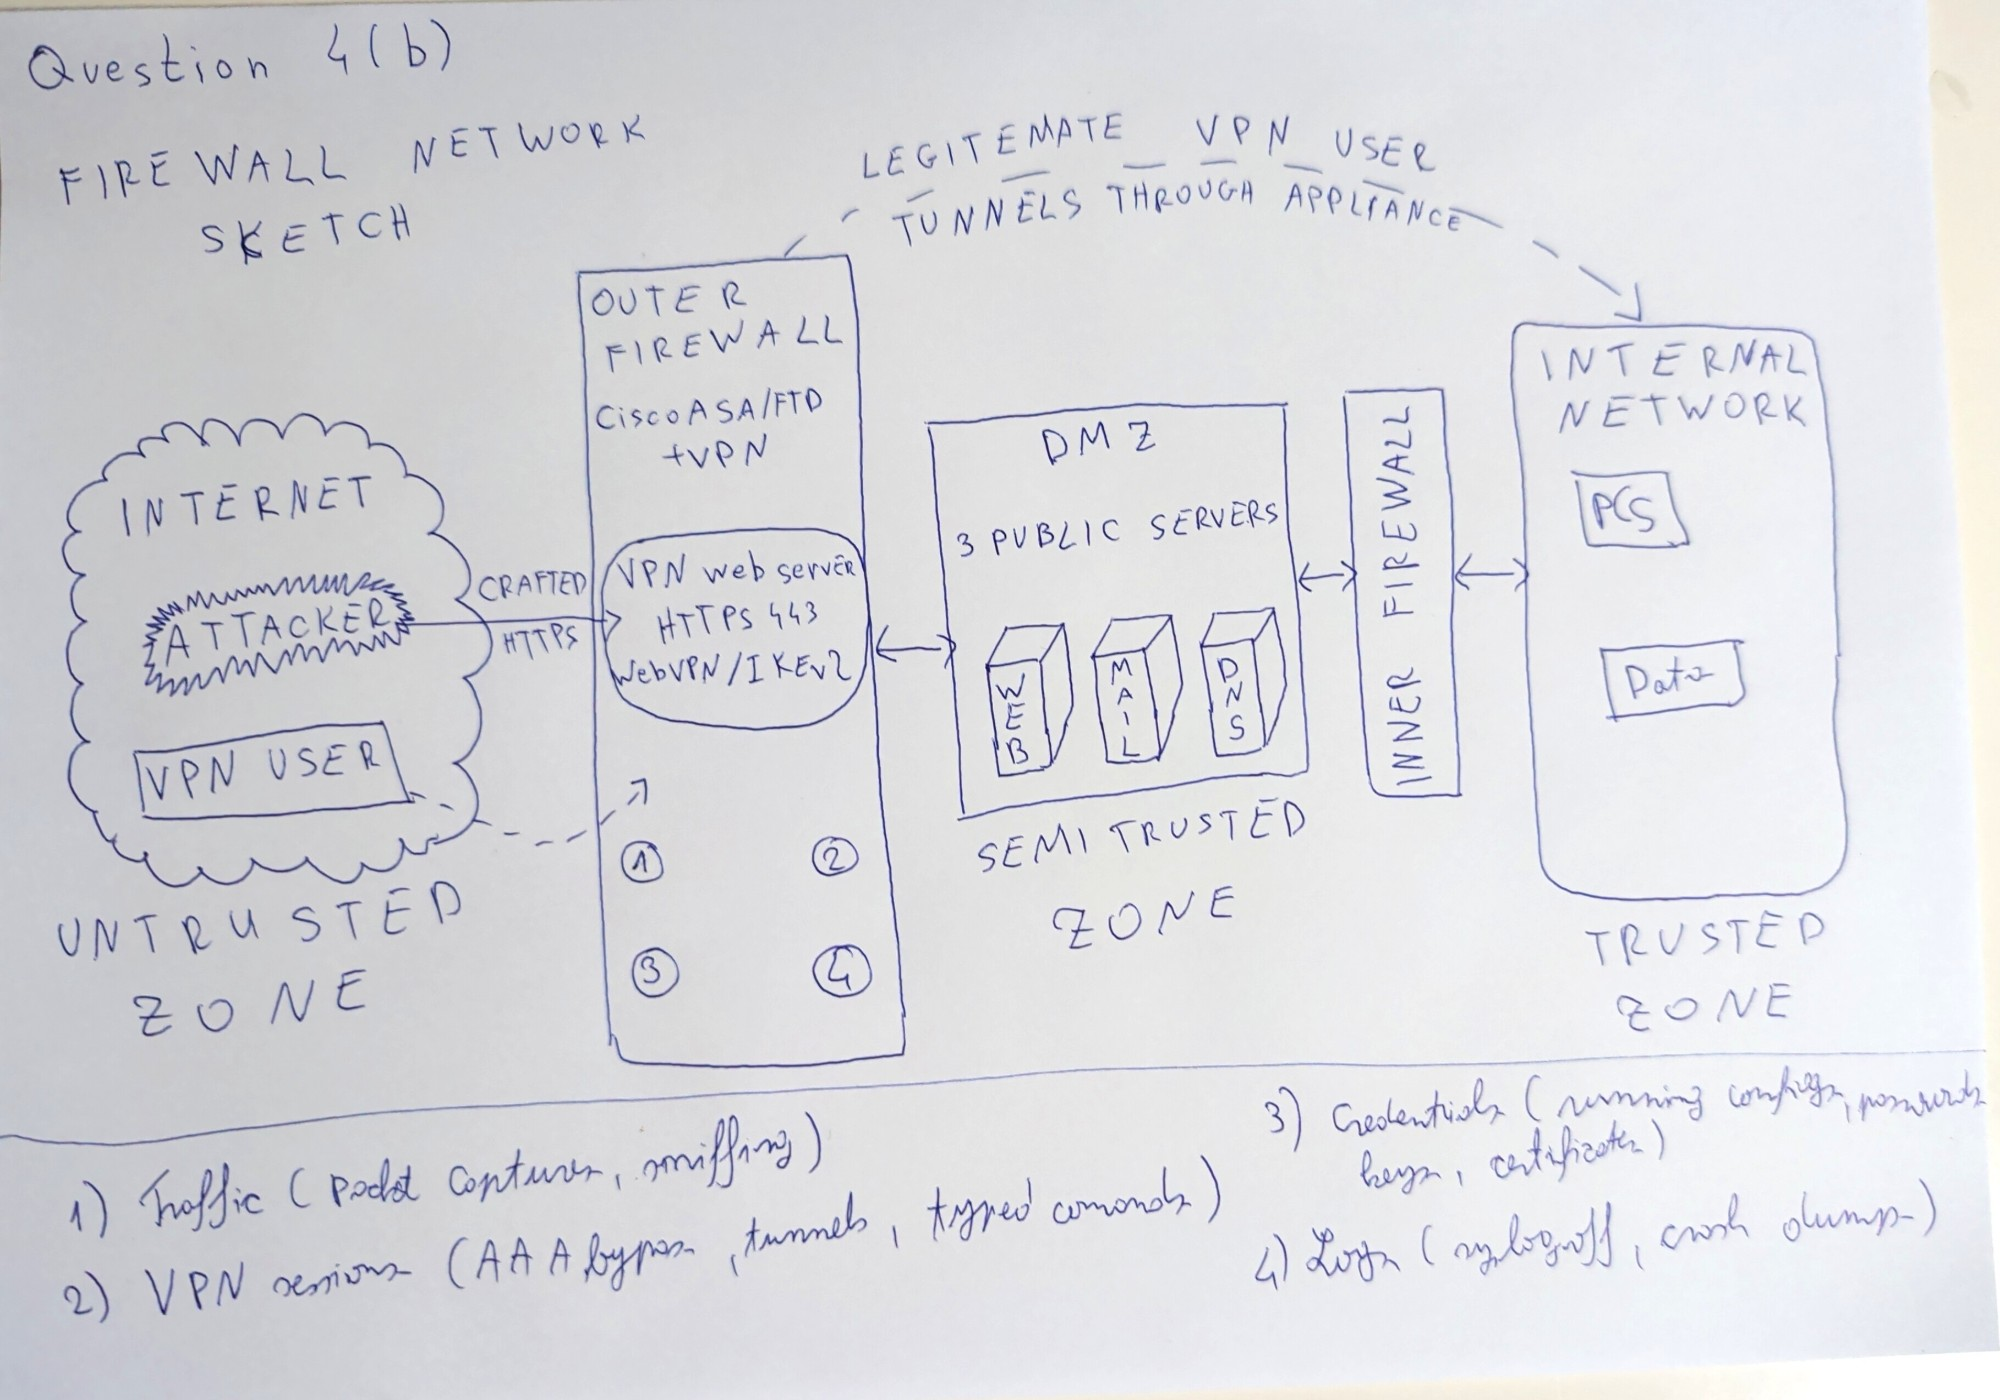
\includegraphics[width=0.92\linewidth]{figures/q4_network_hand_drawn.jpg}}{\fourdiagram}
\IfFileExists{figures/q4_network_hand_drawn.jpg}{%
\caption{Hand drawing: the Internet, the ASA/FTD firewall and VPN appliance as the outer firewall, the DMZ, an inner firewall and the internal network: the DMZ between two firewalls (Stamp \cite{stamp}), with the attacked VPN web server and what an attacker who controls the appliance can see and change.}}{%
\caption{The Internet, the ASA/FTD firewall and VPN appliance as the outer firewall, the DMZ, an inner firewall and the internal network: the DMZ between two firewalls (Stamp \cite{stamp}). The sheet asks for a drawing made by hand; this typeset
version shows what that drawing must contain, and \code{figures/q4\_network\_hand\_drawn.jpg} replaces it when it exists.}}\label{fig:q4net}
\end{figure}
The attacked \textbf{service of the appliance} is its \textbf{remote-access VPN web server}: the HTTPS interface of SSL VPN (WebVPN) and of IKEv2 client services, which must be
reachable from the Internet because remote users connect to it. Devices were vulnerable if a related remote-access VPN configuration was enabled
\cite{ciscoadv,ciscoevent}. An attacker who \emph{controls the appliance} (the 2024 and 2025 implants) can, according to Talos, Cisco and the NCSC
\cite{talos,ciscoevent,ncscmar}:
\begin{itemize}
\item \textbf{see and change traffic}: create and exfiltrate packet captures and sniff network traffic; the appliance is the outer firewall: all traffic between the Internet and the DMZ passes through it, and VPN users enter the network through it;
\item \textbf{see and change VPN sessions}: bypass the AAA (authentication) check for the actor's own devices, establish a VPN tunnel into the network, harvest the commands
that administrators type;
\item \textbf{see and change credentials}: read and export the running configuration, which holds the device's passwords, certificates and keys (Cisco therefore says to treat all
configuration of a compromised device as untrusted and to replace passwords, certificates and keys);
\item \textbf{see and change logs}: disable or suppress syslog messages and alter the crash-dump process so that forensics fail; LINE VIPER also reboots the device when it
detects a memory dump or analysis.
\end{itemize}

\paragraph{(c) Why filtering in front does not solve it, end-of-support devices, secure boot, defence in depth.}
\emph{Why a packet filter, a stateful filter or an application proxy placed in front of the appliance cannot solve the problem.}
(1) The vulnerable component is the service the organisation \emph{wants} to expose: VPN users must reach the HTTPS port of the VPN web server, so a packet filter
(addresses, ports, flags) and a stateful filter (connections) have to allow exactly the traffic that carries the exploit. (2) An application proxy could inspect the
content, but the TLS session ends at the appliance, so the proxy would have to terminate TLS itself, which is not how the remote-access VPN works; and the exploits are
ordinary, well-formed HTTPS requests (CVE-2025-20362 needs no credentials, CVE-2025-20333 only a valid VPN login) \cite{ciscoadv}. (3) The compromised device \emph{is} the perimeter:
once the attacker controls it, a filter in front of it protects the attacker, who can also tamper with the logs that would reveal the intrusion. (4) The implant survives:
filters do not remove a bootkit.

\emph{Why the directive treated devices near their end of support differently.} ED~25-03 ordered ASA hardware whose end of support fell on or before 30~September 2025 to be
\emph{permanently disconnected}, while the other devices were to be updated \cite{ed2503}. The reasons: those models receive no further fixes (the fixed ASA~9.12 and 9.14 releases for the oldest
5500-X models are their last releases, and several models had already passed their last day of support) \cite{ciscoadv,ciscoevent}; the NCSC notes that every targeted model had passed
its last day of support or reached it on 30~September 2025, and that the models were released in 2012 with an end-of-life notice in 2020 \cite{ncscmar}; and, crucially, they have no secure boot, so
a compromise cannot be removed by an update: CISA states that applying Cisco's updates ``does not necessarily remove'' an existing threat actor \cite{ed2503}.

\emph{The role of secure boot.} The NCSC states that the models that were attacked do not use secure boot, so there is no cryptographic verification of early boot software \cite{ncscmar}. The
actor modified the read-only memory (ROMMON, and in the NCSC analysis a GRUB bootkit, RayInitiator) so that the implant persisted across reboots and software upgrades \cite{ciscoevent,ncscmar}. With secure
boot and a hardware trust anchor the early boot stages are verified against a signature before they run, so a modified boot stage is rejected; Cisco reports that it has
not observed successful compromise on platforms with Secure Boot and Trust Anchors \cite{ciscoevent}.

\emph{Relation to defence in depth.} Defence in depth combines layers, such as a DMZ between two firewalls (Stamp \cite{stamp}), so that one failure does not give everything. Here the
perimeter device was the single layer that all others trusted, and its own integrity depended on one layer only. The incident shows which layers were missing around it: a trusted
boot chain (integrity of the device), timely patching, logs stored off the device, separation of the management plane, and inside the network the assumption that traffic from the VPN is not
automatically trusted (Table~\ref{tab:q4layers}).
\begin{table}[H]
\centering\small
\begin{tabularx}{\textwidth}{@{}P{3.5cm}LL@{}}
\toprule
Layer & What it would have done & Evidence from the incident \\
\midrule
Secure boot, hardware trust anchor & rejects a modified ROMMON/GRUB, so the implant cannot persist across reboot and upgrade & the attacked models had none \cite{ncscmar,ciscoevent} \\
Timely patching and end-of-life replacement & closes CVE-2025-20333 and -20362; removes unsupported hardware & directive: patch within 48 hours of release, disconnect end-of-support models \cite{ed2503} \\
Off-device logging & records what a device cannot hide after compromise & the implants suppress syslog and tamper with crash dumps \cite{talos,ncscmar} \\
Segmentation behind the appliance & limits what a VPN tunnel or a captured session reaches & the appliance is only the outer firewall: the DMZ and an inner firewall lie behind it (Figure~\ref{fig:q4net}) \\
\bottomrule
\end{tabularx}
\caption{Layers around the appliance and what the incident shows about them.}\label{tab:q4layers}
\end{table}

\paragraph{(d) Three controls.}
\begin{enumerate}[label=(\arabic*)]
\item \textbf{Limit where the management and VPN web interfaces are exposed.} Allow management access only from a management network or jump host, restrict the VPN endpoint to
what remote users need, and disable VPN web services (for example \code{no webvpn}) and IKEv2 client services on devices that do not use them. \emph{Evidence:} both 2025 CVEs are in the VPN
web server, the attack applies to devices with VPN web services enabled, and Cisco lists disabling these services as a temporary mitigation \cite{ciscoevent,ciscoadv}.
\item \textbf{Store logs off the device and alert when they stop.} Send syslog to a separate collector with its own time source and integrity protection, and treat silence, an unexpected
reload or a crash dump as an event. \emph{Evidence:} Line Dancer disables syslog, LINE VIPER suppresses syslog messages and reboots when it sees analysis, and the crash-dump process is altered to defeat
forensics \cite{talos,ncscmar}; Cisco observed attackers disabling logging, intercepting commands and crashing devices on purpose \cite{ciscoevent}.
\item \textbf{Check the integrity of the device and keep its life cycle under control.} Patch within days, replace end-of-support models and prefer platforms with secure boot, run the
vendor's core-dump and integrity procedure and disconnect a device that shows compromise, then reset it and replace all passwords, certificates and keys. \emph{Evidence:} ED~25-03 requires exactly
this (core dumps, 48-hour updates, disconnecting end-of-support hardware, inventory), and states that an update alone does not remove an existing actor \cite{ed2503}; Cisco tells owners of compromised
devices to reset them and rotate credentials \cite{ciscoevent}.
\end{enumerate}

\subsection*{Question 5 --- A forged key and a custom alert (2023)}

\paragraph{(a) Who, what, when.} The \textbf{cloud provider} is Microsoft (Exchange Online and Outlook.com). The
\textbf{threat actor} is Storm-0558, assessed by Microsoft with moderate confidence to be China-based with
espionage objectives (Microsoft now tracks it as Antique Typhoon) \cite{msanalysis}. The \textbf{department that detected the intrusion} is the
U.S.\ \textbf{Department of State}, and the \textbf{review board} is the \textbf{Cyber Safety Review Board (CSRB)}, which
reviewed the intrusion at the request of the Secretary of Homeland Security and found it ``preventable and should never have
occurred'' \cite{csrb}. The actor reached the mailboxes of 22 organisations and 503 related personal accounts, among them the
Commerce Secretary and the U.S.\ Ambassador to China; about 60\,000 e-mails were taken from the State Department alone \cite{csrb}.
\begin{table}[H]
\centering\small
\begin{tabular}{@{}llP{10.6cm}@{}}
\toprule
\# & Date (UTC) & Event \\
\midrule
1 & 2016 & Microsoft creates the consumer (MSA) signing key later forged; it should have been retired in March 2021, but
retirement was delayed \cite{csrb} \\
2 & 15 May 2023 & intrusion start: Storm-0558 gains access to e-mail accounts using forged tokens \cite{csrb,msanalysis} \\
3 & 15 Jun.\ 2023 & the State Department's security operations centre detects anomalous access to its mail systems \cite{csrb} \\
4 & 16 Jun.\ 2023 & the custom ``Big Yellow Taxi'' alerts are reviewed; State notifies Microsoft \cite{csrb,msanalysis} \\
5 & 11 Jul.\ 2023 & \textbf{Microsoft's first disclosure} of the intrusion (MSRC and ``Microsoft on the Issues'' blogs) \cite{msanalysis} \\
6 & 6 Sep.\ 2023 & \textbf{Microsoft's explanation} of how the key was stolen: a 2021 crash dump moved to a debugging
environment \cite{mskey} \\
7 & 12 Mar.\ 2024 & \textbf{the correction}: Microsoft has found no crash dump containing the key; it does not know how
the key was obtained \cite{mskey,csrb} \\
8 & 20 Mar.\ 2024 & date of the CSRB report \cite{csrb} \\
\bottomrule
\end{tabular}
\caption{Timeline of the Storm-0558 intrusion (gaps computed in Appendix~A.4: 31 days from intrusion to detection, 26 days from detection to
disclosure, 188 days from the inaccurate blog to its correction).}\label{tab:q5time}
\end{table}
The CSRB also notes that Microsoft acknowledged to the Board in November 2023 that the September post was inaccurate, but
corrected it only on 12 March 2024, ``after the Board's repeated questioning'' \cite{csrb}. The window of compromise
may have started earlier than 15~May because of the standard 30-day log retention \cite{csrb}.

\paragraph{(b) How the State Department detected it, and the authentication failure.} State's SOC ran a custom alert rule,
named \textbf{``Big Yellow Taxi''}, over the \textbf{\code{MailItemsAccessed}} audit log, which records access to Exchange Online
mailboxes. The rule enumerated the applications accessing mailboxes, compared them with a baseline, and alerted when an
application ID that did not normally touch mailboxes appeared; the same data was used in CISA's detection guidance, which
asked for unexpected \code{MailItemsAccessed} events with irregular application IDs \cite{csrb,cisa193}. The activity could look
normal, and State had seen false alarms from this rule before, but it investigated and found the intrusion \cite{csrb}.

\emph{Why other victims did not see it:} \code{MailItemsAccessed} is part of Microsoft Purview Audit (Premium), available through
the G5/E5 licences. State had bought the government G5 licence; the Board found that few, if any, other victims had the
enhanced logging, and that even then few organisations analyse the voluminous log in detail \cite{csrb}.

\emph{Signature-based or anomaly-based?} The detection is \textbf{anomaly-based}: it does not look for a known attack pattern
or indicator, it compares mailbox access with a learned baseline of normal applications (the rule is hand-written, but what it
detects is a deviation, and State built it from three years of experience of anomalous mailbox access) \cite{csrb}.

\emph{The authentication failure.} The key that was stolen was a \textbf{Microsoft account (MSA) consumer signing key},
created in \textbf{2016}, so about seven years old, and two years past its planned retirement in March 2021; Microsoft had stopped
rotating consumer keys in 2021 and had no automatic alert on the age of active keys \cite{csrb}. Such a key should have been
able to sign only tokens for consumer Outlook. It worked for enterprise mailboxes because of a \textbf{token validation flaw}:
Microsoft had introduced a common OpenID Connect endpoint that lists the signing keys of both the consumer and the enterprise
identity systems, but had not updated its SDKs to tell the two kinds of key apart, so Exchange Online accepted a token signed
with the consumer key for an enterprise account \cite{csrb,mskey}. Together, the old key and the missing check gave
``full access to essentially any Exchange Online account'' \cite{csrb}.

\paragraph{(c) Base rate.} A monitoring system sees $5\times10^{7}$ events per day, one in $10^{6}$ is malicious, the detection
rate is $\mathrm{TPR}=0.95$, the false positive rate is $\mathrm{FPR}=10^{-3}$, and an analyst investigates 60 alerts per day
(\code{q5\_base\_rate.py}, Appendix~A.3). Let $p=10^{-6}$ and $N=5\times10^{7}$.
\begin{table}[H]
\centering\small
\begin{tabular}{@{}lrl@{}}
\toprule
Quantity & Value & Calculation \\
\midrule
malicious events per day & $50$ & $N\,p$ \\
true alerts & $47.5$ & $N\,p\cdot\mathrm{TPR}$ \\
false alerts & $49\,999.95$ & $N(1-p)\cdot\mathrm{FPR}$ \\
\textbf{alerts per day} & $\mathbf{50\,047.45}$ & $47.5+49\,999.95$ \\
$P(\text{attack}\mid\text{alert})$ & $9.49\times10^{-4}\approx0.095\%$ & $47.5/50\,047.45$, one alert in 1054 is real \\
\textbf{analysts needed} & $\mathbf{835}$ & $50\,047.45/60=834.1$, rounded up \\
\bottomrule
\end{tabular}
\caption{Alerts, precision and staffing for the general detector.}
\end{table}
The same $P$ follows from Bayes' formula $\frac{\mathrm{TPR}\,p}{\mathrm{TPR}\,p+\mathrm{FPR}\,(1-p)}$ (Appendix~A.3). Although 95\% of the attacks are
detected, more than 99.9\% of the alerts are false: the 50 million harmless events multiplied by even a tiny FPR outnumber the
50 real attacks by a thousand to one (the base-rate fallacy). A narrow rule can work better because it attacks exactly this
term. A rule that looks for one pattern only, such as an application ID that has never accessed a mailbox before, may miss many
attacks (lower TPR) but produces almost no false alerts (very low FPR), so analysts spend their 60 alerts a day on mostly real
events. With the illustrative, assumed values $\mathrm{TPR}=0.6$ and $\mathrm{FPR}=10^{-6}$ the script gives 80 alerts per day,
$P=37.5\%$ and 2 analysts. This is what State's rule did: it was written for one threat, tuned over three years, and was
therefore small enough to triage \cite{csrb}.

%=====================================================================
\section*{2.4 Authentication Protocols}

\subsection*{Question 6 --- Half a second too slow: the backdoor in SSH (2024)}

\paragraph{(a) The post, the library, the distributions, the timeline.} On 29~March~2024 (08:51 UTC$-$7) the software engineer
Andres Freund posted \emph{``backdoor in upstream xz/liblzma leading to ssh server compromise''} to the public oss-security
list \cite{freund}. The library is \textbf{liblzma} of \textbf{XZ Utils}, versions \textbf{5.6.0} and \textbf{5.6.1}; the
vulnerability is \textbf{CVE-2024-3094} (CVSS~v3 10.0, critical) \cite{nvd}, and CISA advised downgrading to 5.4.6 \cite{cisaxz}.
\begin{table}[H]
\centering\small
\begin{tabularx}{\textwidth}{@{}P{3.4cm}L@{}}
\toprule
Distribution & Version or channel that shipped the backdoored package \\
\midrule
Debian & unstable (5.6.0-0.1 added 26 Feb.\ 2024; 5.6.1 on 27 Mar.), testing (from 5 Mar.), rolled back on 28 Mar.; stable (bookworm) not affected
\cite{cox,debian} \\
Fedora & Rawhide (5.6.0 or 5.6.1) and the Fedora~40 beta (xz-libs 5.6.0-1.fc40 and 5.6.0-2.fc40); no RHEL version \cite{redhat} \\
openSUSE & Tumbleweed and MicroOS, 7--28 March 2024 \cite{suse} \\
Kali Linux & xz-utils 5.6.0-0.2, available 26--29 March 2024 \cite{kali} \\
\bottomrule
\end{tabularx}
\caption{Distributions that shipped the backdoored xz (rolling and pre-release channels).}\label{tab:distros}
\end{table}
\begin{table}[H]
\centering\small
\begin{tabular}{@{}llP{10.6cm}@{}}
\toprule
\# & Date & Event \\
\midrule
1 & 29 Oct.\ 2021 & first contribution by ``Jia Tan'' to xz-devel, a harmless \code{.editorconfig} patch \cite{cox} \\
2 & 22 Apr.\ 2022 & first of the pressure e-mails to the maintainer, Lasse Collin (from ``Jigar Kumar'', later ``Dennis Ens'') \cite{cox} \\
3 & 29 Jun.\ 2022 & Collin calls Jia Tan ``practically a co-maintainer already'' \cite{cox} \\
4 & 28 Oct.\ 2022 & Jia Tan is added to the Tukaani GitHub organisation; direct commit access follows on 30 Dec.\ \cite{cox} \\
5 & 18 Mar.\ 2023 & Jia Tan tags the first release, v5.4.2 \cite{cox} \\
6 & 23--24 Feb.\ 2024 & the backdoor is merged into binary test files; v5.6.0 is released with the malicious
\code{build-to-host.m4} in its tarball \cite{cox} \\
7 & 9 Mar.\ 2024 & v5.6.1 is released \cite{cox} \\
8 & 28 Mar.\ 2024 & Freund finds the backdoor and tells Debian and distros@openwall privately \cite{cox} \\
9 & 29 Mar.\ 2024 & public disclosure on oss-security; CVE-2024-3094 \cite{freund,nvd} \\
\bottomrule
\end{tabular}
\caption{Timeline of the contributor's involvement (Appendix~A.4: 882 days, 2.4 years, from the first contribution to the
disclosure; 34 days from the backdoored release to the disclosure).}\label{tab:xztime}
\end{table}

\paragraph{(b) How code in a compression library ended up inside the SSH server.}
\begin{table}[H]
\centering\small
\begin{tabular}{@{}lP{3.2cm}P{9.6cm}@{}}
\toprule
\# & Stage & What happens \cite{freund,cox} \\
\midrule
1 & release tarball & the tarball of 5.6.0/5.6.1 contains a modified \code{m4/build-to-host.m4} that is \emph{not} in the git repository \\
2 & build script & \code{configure} runs the macro; it decodes the test file \code{bad-3-corrupt\_lzma2.xz} into a script, which decodes
\code{good-large\_compressed.lzma} and extracts an object file; it acts only for x86-64 Linux, GCC with GNU \code{ld} and a Debian or RPM build \\
3 & library & the object (\code{liblzma\_la-crc64-fast.o}) is linked into \code{liblzma.so}; it replaces the IFUNC resolvers \code{crc32\_resolve()} and
\code{crc64\_resolve()} \\
4 & distribution patch & Debian and several other distributions patch OpenSSH's \code{sshd} for systemd notification; the patch links \code{libsystemd}, which depends on \code{liblzma} \\
5 & SSH server start & \code{sshd} loads \code{liblzma}; because it is built with \code{-Wl,-z,now}, the resolvers run at once and install an audit hook in the dynamic linker \\
6 & redirected function & when \code{RSA\_public\_decrypt@plt} is resolved, the hook points its GOT entry (still writable at that moment) into the backdoor \\
7 & public-key login & \code{ssh\_rsa\_verify} calls the redirected \code{RSA\_public\_decrypt}, which runs the backdoor's check and then calls back into libcrypto \\
\bottomrule
\end{tabular}
\caption{The chain of Figure~\ref{fig:xz} in words.}\label{tab:xzchain}
\end{table}
\begin{figure}[H]
\centering
\IfFileExists{figures/xz_chain_hand_drawn.jpg}{%
  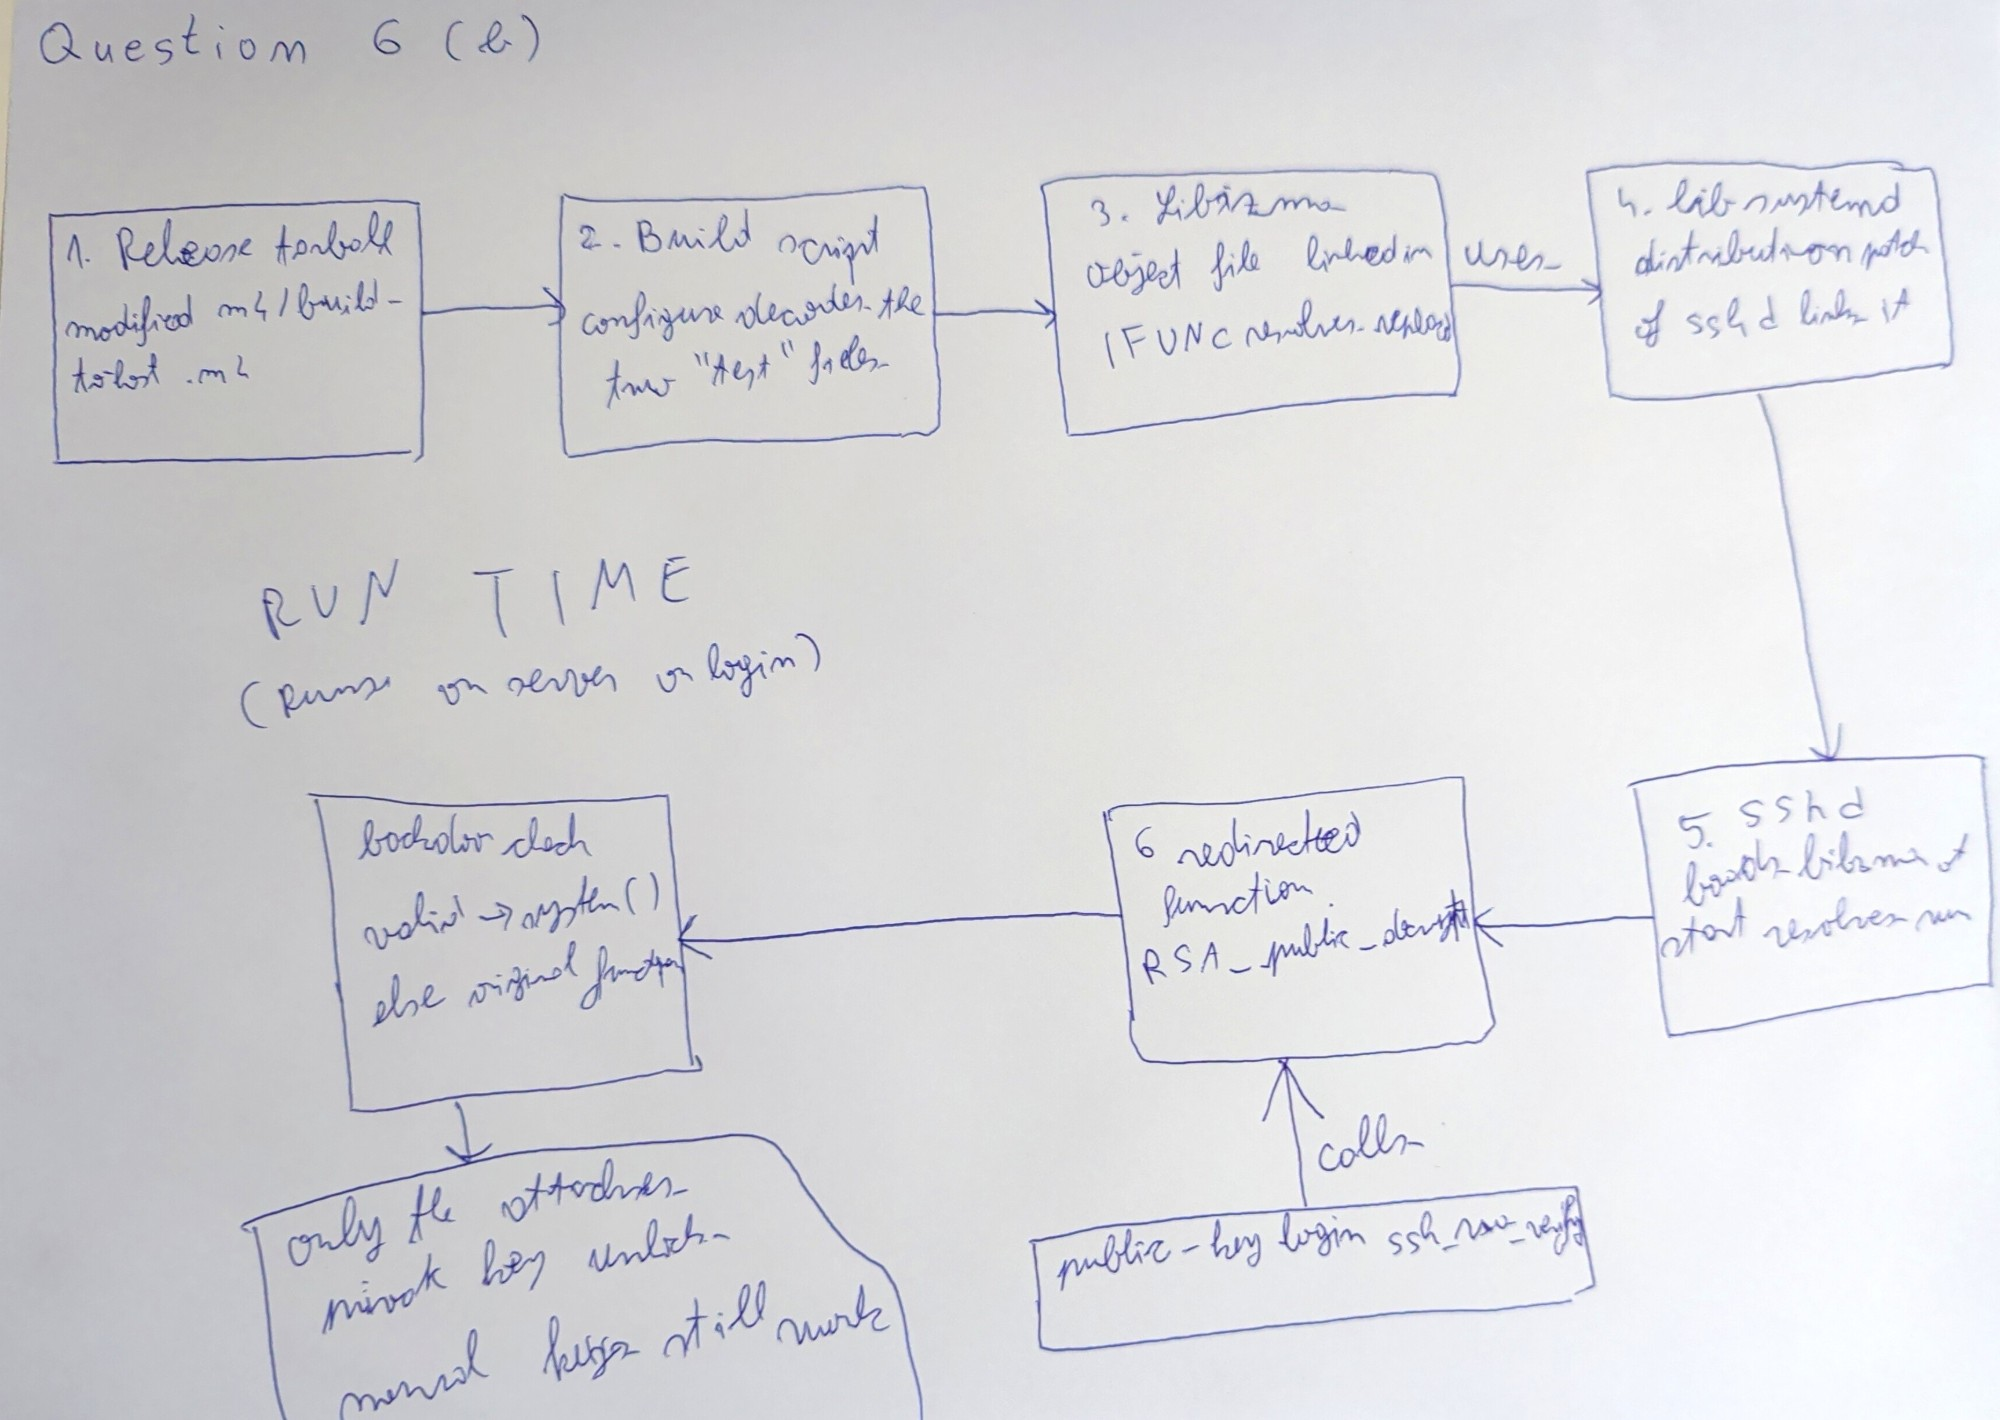
\includegraphics[width=0.92\linewidth]{figures/xz_chain_hand_drawn.jpg}}{\xzdiagram}
\IfFileExists{figures/xz_chain_hand_drawn.jpg}{%
\caption{Hand drawing: the chain from the xz release tarball through the build script, \code{liblzma}, \code{libsystemd} and \code{sshd} to the redirected function \code{RSA\_public\_decrypt}.}}{%
\caption{The chain from the xz release tarball to the SSH server. The sheet asks for a drawing made by hand; this typeset version shows what that drawing
must contain, and \code{figures/xz\_chain\_hand\_drawn.jpg} replaces it when it exists.}}\label{fig:xz}
\end{figure}
\emph{Why the malicious code was in the release tarballs but not in the visible repository.} Distributions build from the
\emph{release tarball} that the maintainer uploads, not from the git tree. The macro that unpacks the payload was added only to
that tarball; the GitHub ``source code'' archives, generated from the repository, do not contain it \cite{freund}. The payload
itself sat in the repository, but disguised as two binary test files (\code{bad-3-corrupt\_lzma2.xz} and
\code{good-large\_compressed.lzma}) that nothing used as tests \cite{freund}. A reviewer reading the repository would see neither the
trigger nor an obviously malicious file.

\paragraph{(c) The authentication protocol, the function, and the violated assumption.} SSH public-key authentication is a
challenge--response protocol: the server asks the client to sign data that includes the session identifier, and the client answers
with a signature made with its private key. The server \emph{verifies} the signature with the user's public key. For an RSA key
\code{ssh\_rsa\_verify} does this through \code{RSA\_public\_decrypt}, which recovers the signed digest from the signature so that
it can be compared \cite{freund}. This is the function the backdoor redirects.

\emph{What the backdoor checked before acting.} Freund himself had not yet worked out what the injected code checks; he
suspected some form of access in a pre-authentication context \cite{freund}. A preliminary analysis by F.~Valsorda, reposted
to oss-security, describes it: the payload is taken from the $N$ value of the RSA public key passed to
\code{RSA\_public\_decrypt}, which an attacker controls before authentication through an OpenSSH certificate (a certificate
carries the signer's public key); it is checked against a simple fingerprint, decrypted with a fixed ChaCha20 key, and its
signature is verified with a fixed Ed448 key; only then is the command handed to \code{system()}. If the payload is malformed or the
signature does not verify, the backdoor reverts to normal operation, so every legitimate login works as before
\cite{patrakov}. It also acts only when the process is \code{/usr/sbin/sshd} with \code{TERM} unset, and it appears to detect
\code{rr} and, in some cases, \code{gdb} \cite{freund}. Only the holder of the attacker's private key can use it, which makes
it a gated remote-code-execution backdoor, not a password bypass.

\emph{Why this is not a weakness of the protocol.} The protocol and its cryptography were not broken: an attacker who did not
have the matching private key could not forge a signature against an honest verifier. The attack \emph{replaced the verifier's code}
and so bypassed the protocol instead of attacking it. \emph{The assumption violated} is the one every authentication protocol
makes about its endpoints: that each party runs the genuine, unmodified implementation of the protocol on a platform it can
trust, so that the check it appears to perform is the check that is performed. A supply-chain compromise breaks exactly that
assumption, which is why the best protocol cannot compensate for it.

\paragraph{(d) The anomaly, and controls.} The discovery was a form of human anomaly detection \cite{freund}. Freund saw that SSH
logins on his Debian unstable test system used a lot of CPU and were slow: \code{time ssh nonexistant@localhost} took 0.299\,s
before and 0.807\,s with the backdoored library, and \code{sshd -h} took about 0.5\,s instead of 0.01\,s, with the user and system
time unchanged. \code{valgrind} reported errors in some configurations (the injected code expected a different stack layout; 5.6.1 was a
workaround). He then used \code{perf record -e intel\_pt//ub} to find where execution diverged with and without the library and
\code{gdb} breakpoints before the divergence \cite{freund}.

Three controls that would make such an attack harder, with evidence from the incident:
\begin{enumerate}[label=(\arabic*)]
\item \textbf{Technical: build from the signed git tag, or build reproducibly, and compare the release tarball with the repository.}
The malicious macro existed only in the tarball \cite{freund}. A check that a tarball equals \code{git archive} of its tag (apart
from listed generated files) would have flagged \code{build-to-host.m4}; Arch Linux changed its package to build from git on
28~March \cite{cox}.
\item \textbf{Technical: remove unneeded dependencies from the authentication daemon, and keep performance tests in the pipeline.}
\code{sshd} was reachable only because distribution patches pulled in \code{libsystemd}, and with it \code{liblzma}
\cite{freund}; since OpenSSH~9.8 systemd notification has a standalone implementation that does not depend on \code{libsystemd}
\cite{openssh98}. The slowdown (0.3\,s to 0.8\,s)
shows that a regression test on login time would also have caught it.
\item \textbf{Non-technical: governance of maintainers.} The campaign worked on a single maintainer under pressure: e-mails
from newly appearing accounts started 175 days after the first contribution, and the contributor was a ``practically a
co-maintainer'' after 243 days \cite{cox}. Two-person review and release signing, shared maintainership, and support for
maintainers (funding, rest) reduce the effect of social pressure.
\end{enumerate}

%=====================================================================
\section*{Conclusion}
The six incidents share one pattern: the attacker spent very little (a 60-byte request, one e-mail, a leaked password, one stolen key, two years of
patience, a vulnerable appliance) and the defender's cost was large (a 201 million requests/s flood, half of an operator's traffic for hours, mailboxes read for about a month before detection,
a firewall that a software update could not clean, 50\,000 false alerts a day). In every case a precise defence existed and was cheap compared with the damage: a second
factor and an alarm on the registry account, bounding the \emph{work} a reset stream can cause, executing no inline script, validating the issuer and scope of every key, verifying the
boot chain of the perimeter device, and building only what the repository contains.

\clearpage
\begin{thebibliography}{99}
\footnotesize\setlength{\itemsep}{1pt}\setlength{\parsep}{0pt}\setlength{\parskip}{0pt}

\bibitem{stamp}
M.~Stamp, \emph{Information Security: Principles and Practice}, 3rd~ed. Hoboken, NJ, USA: Wiley, 2022, chs.~8--9.

\bibitem{ripestat}
RIPE NCC, ``RIPEstat'' (web interface and Data API: \texttt{rpki-validation}, \texttt{announced-prefixes}, \texttt{as-overview}) and RIPE Database (organisation ORG-IA73-RIPE). [Online]. Available:
\url{https://stat.ripe.net/} (accessed Nov.~17, 2026).

\bibitem{record}
J.~Greig and J.~Warminsky, ``Major Spanish mobile carrier suffers three-hour outage after account takeover,'' The Record, Jan.~4, 2024. [Online]. Available:
\url{https://therecord.media/orange-espana-outage-hacker-internet-ripe-bgp-rpki} (accessed Nov.~17, 2026).

\bibitem{ripeupdate}
H.~P.~Holen, ``[News] Security breach: Investigation update,'' RIPE NCC, ncc-announce mailing list, Jan.~10, 2024. [Online]. Available:
\url{https://www.ripe.net/ripe/mail/archives/ncc-announce/2024-January/001695.html} (accessed Nov.~17, 2026).

\bibitem{apnic}
D.~Madory, ``Digging into the Orange Espa\~na hack,'' APNIC Blog (guest post, originally on the Kentik blog), Jan.~26, 2024. [Online]. Available:
\url{https://blog.apnic.net/2024/01/26/digging-into-the-orange-espana-hack/} (accessed Nov.~17, 2026).

\bibitem{rfc6811}
P.~Mohapatra, J.~Scudder, D.~Ward, R.~Bush, and R.~Austein, ``BGP prefix origin validation,'' IETF RFC~6811, Jan.~2013. [Online]. Available:
\url{https://www.rfc-editor.org/rfc/rfc6811}

\bibitem{rfc9319}
Y.~Gilad, S.~Goldberg, K.~Sriram, J.~Snijders, and B.~Maddison, ``The use of maxLength in the Resource Public Key Infrastructure (RPKI),'' IETF RFC~9319 (BCP~185), Oct.~2022. [Online]. Available:
\url{https://www.rfc-editor.org/rfc/rfc9319}

\bibitem{register}
``Weak password and infostealer blamed for Orange Spain outage,'' The Register, Jan.~4, 2024. [Online]. Available:
\url{https://www.theregister.com/2024/01/04/orange_spain_outage_breach/} (accessed Nov.~17, 2026).

\bibitem{ripereport}
RIPE NCC, ``RIPE NCC Access: Security investigation report,'' May~13, 2024. [Online]. Available:
\url{https://www.ripe.net/publications/documentation/disclosures-and-reports/ripe-ncc-access-security-investigation-report/} (accessed Nov.~17, 2026).

\bibitem{nvd}
National Institute of Standards and Technology, ``National Vulnerability Database: CVE-2023-44487, CVE-2020-35730, CVE-2023-43770,
CVE-2024-11182, CVE-2024-27443, CVE-2024-3094, CVE-2024-20353, CVE-2024-20359, CVE-2025-20333, CVE-2025-20362.'' [Online]. Available: \url{https://nvd.nist.gov/vuln/detail/CVE-2023-44487} (and the same path
for the other identifiers) (accessed Nov.~17, 2026).

\bibitem{cfzero}
Cloudflare, ``HTTP/2 Zero-Day vulnerability results in record-breaking DDoS attacks,'' Cloudflare Blog, Oct.~10, 2023. [Online]. Available:
\url{https://blog.cloudflare.com/zero-day-rapid-reset-http2-record-breaking-ddos-attack/} (accessed Nov.~17, 2026).

\bibitem{cftech}
Cloudflare, ``HTTP/2 Rapid Reset: Deconstructing the record-breaking attack,'' Cloudflare Blog, Oct.~10, 2023. [Online]. Available:
\url{https://blog.cloudflare.com/technical-breakdown-http2-rapid-reset-ddos-attack/} (accessed Nov.~17, 2026).

\bibitem{googlehow}
Google Cloud, ``How it works: The novel HTTP/2 `Rapid Reset' DDoS attack,'' Google Cloud Blog, Oct.~10, 2023. [Online]. Available:
\url{https://cloud.google.com/blog/products/identity-security/how-it-works-the-novel-http2-rapid-reset-ddos-attack} (accessed Nov.~17, 2026).

\bibitem{google398}
Google Cloud, ``Google Cloud mitigated largest DDoS attack, peaking above 398 million rps,'' Google Cloud Blog, Oct.~10, 2023. [Online]. Available:
\url{https://cloud.google.com/blog/products/identity-security/google-cloud-mitigated-largest-ddos-attack-peaking-above-398-million-rps} (accessed Nov.~17, 2026).

\bibitem{aws}
T.~Scholl and M.~Ryland, ``How AWS protects customers from DDoS events,'' AWS Security Blog, Oct.~10, 2023. [Online]. Available:
\url{https://aws.amazon.com/blogs/security/how-aws-protects-customers-from-ddos-events/} (accessed Nov.~17, 2026).

\bibitem{cf71}
Cloudflare, ``Cloudflare mitigates record-breaking 71 million request-per-second DDoS attack,'' Cloudflare Blog, Feb.~13, 2023. [Online]. Available:
\url{https://blog.cloudflare.com/cloudflare-mitigates-record-breaking-71-million-request-per-second-ddos-attack/} (accessed Nov.~17, 2026).

\bibitem{rfc9113}
M.~Thomson and C.~Benfield, ``HTTP/2,'' IETF RFC~9113, Jun.~2022, \S5.1.2. [Online]. Available: \url{https://www.rfc-editor.org/rfc/rfc9113}

\bibitem{godb}
Go Project, ``GO-2023-2102: Excessive resource consumption by rapid HTTP/2 stream resets (CVE-2023-39325),'' Go Vulnerability Database, Oct.~2023. [Online]. Available:
\url{https://pkg.go.dev/vuln/GO-2023-2102} (accessed Nov.~17, 2026).

\bibitem{eset}
M.~Faou, ``Operation RoundPress targeting high-value webmail servers,'' ESET Research, WeLiveSecurity, May~15, 2025. [Online]. Available:
\url{https://www.welivesecurity.com/en/eset-research/operation-roundpress/} (accessed Nov.~17, 2026).

\bibitem{mdn}
MDN Web Docs, ``Content Security Policy (CSP),'' Mozilla. [Online]. Available:
\url{https://developer.mozilla.org/en-US/docs/Web/HTTP/Guides/CSP} (accessed Nov.~17, 2026).

\bibitem{ed2503}
Cybersecurity and Infrastructure Security Agency, ``ED 25-03: Identify and mitigate potential compromise of Cisco devices,'' Emergency Directive, Sep.~25, 2025 (updated Apr.~23, 2026). [Online]. Available:
\url{https://www.cisa.gov/news-events/directives/ed-25-03-identify-and-mitigate-potential-compromise-cisco-devices} (accessed Nov.~17, 2026).

\bibitem{ciscoevent}
Cisco, ``Cisco event response: Continued attacks against Cisco firewalls,'' Sep.~25, 2025 (updated Apr.~24, 2026). [Online]. Available:
\url{https://sec.cloudapps.cisco.com/security/center/resources/asa_ftd_continued_attacks} (accessed Nov.~17, 2026).

\bibitem{ciscoadv}
Cisco, ``Cisco Secure Firewall ASA software and Secure Firewall Threat Defense software VPN web server remote code execution vulnerability,'' Security Advisory cisco-sa-asaftd-webvpn-z5xP8EUB, Sep.~25, 2025. [Online]. Available:
\url{https://sec.cloudapps.cisco.com/security/center/content/CiscoSecurityAdvisory/cisco-sa-asaftd-webvpn-z5xP8EUB} (accessed Nov.~17, 2026).

\bibitem{talos}
Cisco Talos, ``ArcaneDoor: New espionage-focused campaign found targeting perimeter network devices,'' Talos Intelligence Blog, Apr.~24, 2024 (updated Sep.~25, 2025). [Online]. Available:
\url{https://blog.talosintelligence.com/arcanedoor-new-espionage-focused-campaign-found-targeting-perimeter-network-devices/} (accessed Nov.~17, 2026).

\bibitem{secweek}
I.~Arghire, ``Cisco firewall zero-days exploited in China-linked ArcaneDoor attacks,'' SecurityWeek, Sep.~26, 2025. [Online]. Available:
\url{https://www.securityweek.com/cisco-firewall-zero-days-exploited-in-china-linked-arcanedoor-attacks/} (accessed Nov.~17, 2026).

\bibitem{ncscmar}
UK National Cyber Security Centre, ``RayInitiator \& LINE VIPER,'' Malware Analysis Report, version~1.1, Oct.~2025. [Online]. Available:
\url{https://www.ncsc.gov.uk/static-assets/documents/malware-analysis-reports/RayInitiator-LINE-VIPER/ncsc-mar-rayinitiator-line-viper.pdf} (accessed Nov.~17, 2026).

\bibitem{msanalysis}
Microsoft Threat Intelligence, ``Analysis of Storm-0558 techniques for unauthorized email access,'' Microsoft Security Blog, Jul.~14, 2023 (updated Aug.~2024). [Online]. Available:
\url{https://www.microsoft.com/en-us/security/blog/2023/07/14/analysis-of-storm-0558-techniques-for-unauthorized-email-access/} (accessed Nov.~17, 2026).

\bibitem{csrb}
Cyber Safety Review Board, ``Review of the Summer 2023 Microsoft Exchange Online Intrusion,'' U.S.\ Dept.\ Homeland Security, Mar.~20, 2024. [Online]. Available:
\url{https://www.cisa.gov/sites/default/files/2025-03/CSRBReviewOfTheSummer2023MEOIntrusion508.pdf} (accessed Nov.~17, 2026).

\bibitem{mskey}
Microsoft Security Response Center, ``Results of major technical investigations for Storm-0558 key acquisition,'' Sep.~6, 2023 (updated Mar.~12, 2024). [Online]. Available:
\url{https://www.microsoft.com/en-us/msrc/blog/2023/09/results-of-major-technical-investigations-for-storm-0558-key-acquisition} (accessed Nov.~17, 2026).

\bibitem{cisa193}
Cybersecurity and Infrastructure Security Agency and Federal Bureau of Investigation, ``Enhanced monitoring to detect APT activity targeting Outlook Online,'' Alert AA23-193A, Jul.~12, 2023. [Online]. Available:
\url{https://www.cisa.gov/news-events/cybersecurity-advisories/aa23-193a} (accessed Nov.~17, 2026).

\bibitem{freund}
A.~Freund, ``backdoor in upstream xz/liblzma leading to ssh server compromise,'' oss-security mailing list, Mar.~29, 2024. [Online]. Available:
\url{https://www.openwall.com/lists/oss-security/2024/03/29/4} (accessed Nov.~17, 2026).

\bibitem{cisaxz}
Cybersecurity and Infrastructure Security Agency, ``Reported supply chain compromise affecting XZ Utils data compression library, CVE-2024-3094,'' Alert, Mar.~29, 2024. [Online]. Available:
\url{https://www.cisa.gov/news-events/alerts/2024/03/29/reported-supply-chain-compromise-affecting-xz-utils-data-compression-library-cve-2024-3094} (accessed Nov.~17, 2026).

\bibitem{cox}
R.~Cox, ``Timeline of the xz open source attack,'' research!rsc, 2024. [Online]. Available: \url{https://research.swtch.com/xz-timeline} (accessed Nov.~17, 2026).

\bibitem{debian}
Debian Security Team, ``CVE-2024-3094,'' Debian Security Tracker. [Online]. Available:
\url{https://security-tracker.debian.org/tracker/CVE-2024-3094} (accessed Nov.~17, 2026).

\bibitem{redhat}
Red Hat, ``Urgent security alert for Fedora 40 and Fedora Rawhide users,'' Red Hat Blog, Mar.~29, 2024 (updated Mar.~30, 2024). [Online]. Available:
\url{https://www.redhat.com/en/blog/urgent-security-alert-fedora-41-and-rawhide-users} (accessed Nov.~17, 2026).

\bibitem{suse}
M.~Meissner, ``openSUSE addresses supply chain attack against xz compression library,'' openSUSE News, Mar.~29, 2024. [Online]. Available:
\url{https://news.opensuse.org/2024/03/29/xz-backdoor/} (accessed Nov.~17, 2026).

\bibitem{kali}
Kali Linux, ``All about the xz-utils backdoor,'' Kali Linux Blog, Mar.~29, 2024. [Online]. Available:
\url{https://www.kali.org/blog/about-the-xz-backdoor/} (accessed Nov.~17, 2026).

\bibitem{patrakov}
A.~E.~Patrakov (quoting F.~Valsorda's preliminary analysis), ``Re: backdoor in upstream xz/liblzma leading to ssh server compromise,'' oss-security mailing list, Mar.~31, 2024. [Online]. Available:
\url{https://www.openwall.com/lists/oss-security/2024/03/30/36} (accessed Nov.~17, 2026).

\bibitem{openssh98}
OpenSSH Project, ``OpenSSH 9.8 release notes,'' 2024. [Online]. Available: \url{https://www.openssh.org/txt/release-9.8} (accessed Nov.~17, 2026).

\end{thebibliography}

\clearpage
\section*{Appendix A --- Python Verification: Chosen Values and Outputs}
The scripts are in the repository \url{https://github.com/Diellart-Mulolli/network_lab} (see its README for the running guide)
and use only the Python~3 standard library. They were run with Python~3.12.3; the outputs below are included from the
files in \code{outputs/} and are unchanged. Key results were checked a second way: the route validation of Question~1 against the RIPEstat validation of
the same ROAs (Table~\ref{tab:q1today}), the bandwidth figures of Question~2 in two orders (total first, per bot first), the stream model against its closed forms,
and the base rate of Question~5 by counting events and by Bayes' formula.

\needspace{12cm}
\subsection*{A.1 \texttt{q1\_rov.py} (Question 1(b))}
Chosen values: the four phases of the ROAs of the incident (none; the attacker's ROAs for AS49581 of 14:20 UTC; Orange's ROAs for AS12479 with maxLength 12 and 16
after the recovery; maxLength 24 after 8~January 16:00 UTC), five real announcements of AS12479 (two /12s and /16 blocks and three /24s inside them), and the
loss figures of Kentik (9\,200 to 7\,400 routes; 7 to 5 million addresses). Command: \texttt{python3 q1\_rov.py}
\VerbatimInput[fontsize=\footnotesize, frame=single]{outputs/q1_rov.txt}
\textbf{Check.} Phase~1 makes every route Invalid; in phase~2 the /12 and /16 are Valid but the /24s are Invalid (longer than maxLength), and in phase~3 all are Valid, as
reported by APNIC for 3 and 8 January. The loss of 1\,800 routes (19.6\%) and of 2~million addresses (28.6\%) agree with Question~1(b).

\clearpage
\needspace{13cm}
\subsection*{A.2 \texttt{q2\_rapid\_reset.py} (Question 2)}
Chosen values: peak $201\times10^{6}$ requests/s, previous record $71\times10^{6}$, 20\,000 bots, 60 bytes per cancelled
request, 20\,000 bytes per response, stream limit 100, round-trip time 50\,ms. Command: \texttt{python3 q2\_rapid\_reset.py}
\VerbatimInput[fontsize=\footnotesize, frame=single]{outputs/q2_rapid_reset.txt}
\textbf{Check.} The factor 2.83, 10\,050 requests/s per bot, 96.48\,Gbit/s and 4.824\,Mbit/s, 32.16\,Tbit/s and 1.608\,Gbit/s agree
with Question~2(a) and 2(c); the totals computed per bot equal those computed in total; the stream model reproduces the closed forms
$100/0.05=2000$ and $4.824\cdot10^{6}/480=10\,050$.

\needspace{15cm}
\subsection*{A.3 \texttt{q5\_base\_rate.py} (Question 5(c))}
Chosen values: $N=5\times10^{7}$ events/day, $p=10^{-6}$, TPR 0.95, FPR $10^{-3}$, 60 alerts per analyst per day; the narrow-rule
example uses TPR 0.6 and FPR $10^{-6}$ (assumed, for illustration). Command: \texttt{python3 q5\_base\_rate.py}
\VerbatimInput[fontsize=\footnotesize, frame=single]{outputs/q5_base_rate.txt}
\textbf{Check.} 50\,047.45 alerts per day, $P(\text{attack}\mid\text{alert})=9.49\times10^{-4}$ and 835 analysts agree with
Question~5(c); the counting method and Bayes' formula give the same probability (difference 0.0).

\clearpage
\needspace{18cm}
\subsection*{A.4 \texttt{timelines.py} (Questions 1, 4, 5 and 6)}
Chosen values: the dated events of Tables~\ref{tab:q1time}, \ref{tab:q4time}, \ref{tab:q5time} and~\ref{tab:xztime} and the exposure windows of
Table~\ref{tab:distros}; events given only to the month are marked with a tilde and counted from the first of the month. Command: \texttt{python3 timelines.py}
\VerbatimInput[fontsize=\footnotesize, frame=single, firstline=1, lastline=35]{outputs/timelines.txt}
\needspace{17cm}
\VerbatimInput[fontsize=\footnotesize, frame=single, firstline=36, lastline=78]{outputs/timelines.txt}
\textbf{Check.} The gaps quoted in the report are those printed here: 3.7 hours, 8.5 hours and about 5 days for Question~1; 519 days, 818 days and one day for Question~4;
31, 26 and 188 days for Question~5; 882 days, 343 days and 34 days for Question~6.

\end{document}
